\pdfoutput=1
\documentclass[10pt,letterpaper]{article}
%\usepackage{savetrees}
\usepackage[margin=1.2cm]{geometry}
\usepackage{xcolor}
\usepackage{microtype}
\usepackage{amsmath}
\usepackage{amsfonts}
\usepackage{amssymb}
\usepackage{mathtools}
\usepackage{array}
\usepackage{booktabs}
\usepackage{multirow}
\usepackage{bbm}
\usepackage{hyperref}
\usepackage[only, llbracket, rrbracket]{stmaryrd}
\usepackage{latexsym}
\usepackage{expl3,xparse}
\usepackage{tikz}
\usetikzlibrary{automata, arrows, calc, decorations.markings, decorations.pathreplacing, intersections,
  matrix, patterns, positioning, shapes, shapes.geometric, shapes.misc, topaths}
\tikzset{->-/.style = {
    decoration = {markings, mark = at position #1 with {\arrow{>}}},
    postaction = {decorate}}}
\newcommand{\mathtikz}[2][]{\begin{tikzpicture}[baseline=\the\dimexpr-\fontdimen22\textfont2\relax,#1]#2\end{tikzpicture}}
\usepackage{stackengine}
\usepackage{etoolbox}
%\usepackage{mathabx}
\usepackage{graphicx}
\usepackage{enumitem}
\usepackage{etoc}
\usepackage{slashed}

\setlist[itemize]{nosep}
\newcommand*{\myetocenumeratesetup}{}
\protected\def\myetocenumeratesetup{%
  \setlist[enumerate]{label=\etocnumber,
    topsep=0pt,parsep=0pt,partopsep=0pt,itemsep=0pt,
    rightmargin=0pt,
    leftmargin=0pt,
    labelindent=0pt,
    labelsep=0pt,
    align=left,
  }%
  \sloppy\raggedright}
% leftmargin + itemindent = labelindent + labelwidth + labelsep

\setcounter{tocdepth}{5}
\etocmulticolstyle[2]{\myetocenumeratesetup\setlength{\columnsep}{10pt}\setlength{\columnseprule}{.4pt}}
\etocsetstyle{section}
  {\begin{enumerate}[labelwidth=14pt,leftmargin=14pt]}
  {\footnotesize\normalfont\bfseries\item}
  {\etocname{}\nobreak\hfill\etocpage}
  {\end{enumerate}}
\etocsetstyle{subsection}
  {}
  {\scriptsize\normalfont\item}
  {\etocname{} \hbox{}\nobreak\hfill\etocpage}
  {}
\etocsetstyle{subsubsection} % produced by \paragraph, sorry
  {\begin{enumerate}[leftmargin=-8pt]}
  {\tiny\normalfont\item}
  {\etocname{}}
  {\end{enumerate}}
\etocsetstyle{paragraph}{\ERROR}{}{}{}
\etocsetstyle{subparagraph}{\ERROR}{}{}{}

\hypersetup{unicode}
\hypersetup{linktoc = all}                % hyperref settings
\hypersetup{hidelinks}
\pdfstringdefDisableCommands{%
  \def\({}%
  \def\){}%
  \def\\{}%
  \def\pi{\003\300}%
  \edef\sb{\string _}%
  \def\leq{\042\144}%
  \def\infty{\042\036}%
  \def\Tr{Tr }%
}

\setcounter{secnumdepth}{2}
\makeatletter
\ExplSyntaxOn
\cs_generate_variant:Nn \str_head:n { o }
\cs_generate_variant:Nn \clist_if_in:NnT { Nx }
\tl_new:N \l__my_main_tl
\tl_new:N \l__my_title_tl
\cs_set:Npn \__my_first_word_string:w #1 ~ #2 \q_stop { \tl_to_str:n {#1} }
\cs_set:Npn \__my_rest_words:w #1 ~ #2 \q_stop { \exp_not:n {#2} }
\cs_set_protected:Npn \__my_strip_punct:nn #1#2
  {
    \str_case:nnT {#1}
      { { . } { } { : } { } { , } { } { ; } { } }
      {
        \cs_set_protected:Npn \__my_strip:w ##1 #1 \q_nil
          { \tl_set:Nn \l__my_title_tl {##1} }
        \tl_if_in:nnT { #2 \q_nil } { #1 \q_nil } % being paranoid
          { \__my_strip:w #2 \q_nil }
      }
  }
\cs_generate_variant:Nn \__my_strip_punct:nn { xV }
\cs_generate_variant:Nn \use:nn { nx }
\cs_generate_variant:Nn \tl_upper_case:n { f }
\cs_set_eq:NN \__my_strip:w ?
\cs_new_eq:NN \__my_old_sect:w \@sect
\clist_new:N \g_my_omitted_first_words_clist
\clist_gset:Nn \g_my_omitted_first_words_clist { A , The }
\msg_new:nnn { my } { unexpected } { "#1" }
\cs_new:Npn \__my_alphanumeric:N #1
  {
    \quark_if_recursion_tail_stop:N #1
    \int_compare:nF { `a <= `#1 <= `z }
      { \int_compare:nF { `A <= `#1 <= `Z } { \int_compare:nT { `0 <= `#1 <= `9 } } } #1
    \__my_alphanumeric:N
  }
\tl_new:N \l__my_label_tl
\cs_set:Npn \@sect #1 #2 #3 #4 #5 #6 [#7] #8
  {
    \bool_if:nF
      {
        \tl_if_head_eq_meaning_p:nN {#8} \Sectionformat
        && \int_compare_p:n { \tl_count:n {#8} == 3 }
      }
      { \msg_error:nnn { my } { unexpected } {#8} }
    \tl_set:Nx \l__my_main_tl { \tl_item:nn {#8} {2} }
    \tl_set:Nn \l__my_title_tl {#7}
    \tl_if_eq:NNT \l__my_main_tl \l__my_title_tl
      {
        \tl_if_in:NnT \l__my_title_tl { ~ }
          {
            \clist_if_in:NxT \g_my_omitted_first_words_clist
              { \exp_after:wN \__my_first_word_string:w \l__my_title_tl \q_stop }
              {
                \tl_set:Nx \l__my_title_tl
                  { \exp_after:wN \__my_rest_words:w \l__my_title_tl \q_stop }
                \tl_set:Nx \l__my_title_tl
                  {
                    \tl_upper_case:f { \tl_head:N \l__my_title_tl }
                    \tl_tail:N \l__my_title_tl
                  }
              }
          }
        \__my_strip_punct:xV { \tl_item:Nn \l__my_title_tl {-1} }
          \l__my_title_tl
      }
    \tl_set:Nx \l__my_label_tl
      {
        \exp_args:NNf \use:nn \__my_alphanumeric:N % exp_last_unbraced unsafe if empty title
          { \tl_to_str:N \l__my_title_tl }
        \q_recursion_tail \q_recursion_stop
      }
    \use:nx
      { \__my_old_sect:w {#1} {#2} {#3} {#4} {#5} {#6} }
      { [{ \exp_not:V \l__my_title_tl }] } {\label{\l__my_label_tl}#8}
  }
\ExplSyntaxOff
\renewcommand{\section}{\pagebreak[1]\@startsection {section}{1}{\z@ }{-\medskipamount}{\smallskipamount}{\normalfont \large \bfseries \noindent\S}}
\renewcommand{\subsection}{\pagebreak[0]\@startsection {subsection}{2}{\z@ }{-\smallskipamount}{1sp}{\normalfont \large \bfseries \noindent\S}}
\renewcommand{\subsubsection}{\ERROR}
\newcommand{\@@ignorespaces}{}
\let\@@ignorespaces\ignorespaces
\renewcommand{\paragraph}{%
 \def\ignorespaces{\leavevmode\let\ignorespaces\@@ignorespaces}%
 \@startsection {subsubsection}{3}{\z@ }{-\smallskipamount}{-1sp}{\normalfont \bfseries }}
\makeatother
\setlength{\parskip}{2pt plus 2pt minus 2pt}
\setlength{\baselineskip}{10pt}
\setlength{\parindent}{10pt}
\setlength{\hfuzz}{1pt}
\setlength{\vfuzz}{5pt}

\newcommand{\tabfoot}[1]{\leavevmode\ensuremath{{}^{\tabfootsymb{#1}}}}
\makeatletter
\newcommand{\tabfootsymb}[1]{\ensuremath{\scriptstyle\@fnsymbol{\the\numexpr(#1)+2\relax}}}
\makeatother
\newcommand{\caution}[1]{{\scriptsize\mathtikz{\draw (0,-.15)--(.3,-.15)--(.15,.2)--cycle;\node at (.15,0) {!};} #1}}

%%%%%%%%%%%%%%%%%%%%%%%%%%%%%%
% http://tex.stackexchange.com/questions/14386/importing-a-single-symbol-from-a-different-font
\DeclareFontFamily{U}{mathb}{\hyphenchar\font45}
\DeclareFontShape{U}{mathb}{m}{n}{
      <5> <6> <7> <8> <9> <10> gen * mathb
      <10.95> mathb10 <12> <14.4> <17.28> <20.74> <24.88> mathb12
      }{}
\DeclareSymbolFont{mathb}{U}{mathb}{m}{n}
\DeclareFontSubstitution{U}{mathb}{m}{n}
\DeclareMathSymbol{\righttoleftarrow}{3}{mathb}{"FD}
%%%%%%%%%%%%%%%%%%%%%%%%%%%%%%

%\newcommand{\defined}[1]{\textsl{#1}}
\newcommand{\actson}{\mathrel{\reflectbox{$\righttoleftarrow$}}}
\newcommand{\dd}[2][]{\mathop{\mathrm{d}\mkern0mu\relax#1#2}\nolimits}%\mkern avoids \mathop{d} (vertical placement issue)
\newcommand{\DD}[2][]{\mathop{\mathrm{D}\mkern0mu\relax#1#2}\nolimits}%\mkern avoids \mathop{d} (vertical placement issue)
\newcommand{\ie}{i.e.\@}
\newcommand{\eg}{e.g.\@}
\newcommand{\Eg}{E.g.\@}
\makeatletter
\newcommand{\etc}{etc.\@ifnextchar.{\@gobble}{\@}}
\makeatother
\newcommand{\I}{\mathrm{i}}
\newcommand{\rme}{\mathrm{e}}
\newcommand{\Wedge}{\bigwedge}
\newcommand{\Acal}{\mathcal{A}}
\newcommand{\Operator}{\mathcal{O}}
\newcommand{\Chargeconjugation}{\mathcal{C}}
\newcommand{\del}{\partial}
\newcommand{\delbar}{\overline{\partial}}
\newcommand{\Nsusy}{{\mathcal{N}}}
\newcommand{\repr}[1]{\mathbb{#1}}
\newcommand{\todo}[1]{\emph{todo: #1}}
\newcommand{\cyclic}[1]{\ZZ_{#1}}
\newcommand{\ZZ}{\mathbb{Z}} % integers
\newcommand{\QQ}{\mathbb{Q}} % rationals
\newcommand{\RR}{\mathbb{R}} % reals
\newcommand{\CC}{\mathbb{C}} % complex
\newcommand{\HH}{\mathbb{H}} % quaternions
\newcommand{\PP}{\mathbb{P}} % projective
\newcommand{\FF}{\mathbb{F}} % finite field
\newcommand{\torus}{\mathbf{T}} % torus
\DeclarePairedDelimiter{\abs}{\lvert}{\rvert}
\renewcommand{\Im}{}\renewcommand{\Re}{}\let\Im\relax\let\Re\relax
\DeclareMathOperator{\Im}{Im}
\DeclareMathOperator{\Re}{Re}
\DeclareMathOperator{\Hom}{Hom}
\DeclareMathOperator{\Weyl}{Weyl}
\DeclareMathOperator{\End}{End}
\DeclareMathOperator{\Tr}{Tr}
\DeclareMathOperator{\plexp}{plexp}
\DeclareMathOperator{\rank}{rank}
\DeclareMathOperator{\gr}{gr}
\DeclareMathOperator{\diag}{diag}
\DeclareMathOperator{\Li}{Li}
\DeclareMathOperator{\sign}{sign}
\newcommand{\one}{\mathbbm{1}}
\newcommand{\pullback}[2]{#1^*#2}
\newcommand{\bundle}{\mathcal}
\newcommand{\Nf}{N_f}
\newcommand{\thetafunction}{\theta}
\newcommand{\thetaangle}{\theta}
\newcommand{\thetacoordinate}{\theta}
\newcommand{\cardinal}[1]{\abs{#1}}

\ExplSyntaxOn
\NewDocumentCommand{\Lie}{m}{
  \textup
  {
    \clist_if_in:nnF
      { GL , PGL , SL , PSL , SO , PSO , SU , PSU , U , PU , O , PO , Sp , PSp , USp , PUSp , OSp , POSp , Spin , PSpin , Pin, P , PS , A , B , C , D , E , F , G , Q , UQ , W , S , \tilde S , \tilde{S} , H , T }
      {#1} { \UnknownLie }
    #1
  }
}
\NewDocumentCommand{\lie}{m}{
  \mathfrak
  {
    \str_case:nnF {#1}
      {
        { gl } { gl }
        { sl } { sl }
        { so } { so }
        { su } { su }
        { u } { u }
        { o } { o }
        { sp } { sp }
        { usp } { usp }
        { osp } { osp }
        { A } { a }
        { B } { b }
        { C } { c }
        { D } { d }
        { E } { e }
        { F } { f }
        { G } { g }
        { P } { p }
        { Q } { q }
        { UQ } { uq }
        { W } { w }
        { S } { s }
        { \tilde S } { \tilde s }
        { \tilde{S} } { \tilde{s} }
        { H } { h }
        { T } { t }
        { g } { g }
      } { \ERROR #1 }
  }
}
\pdfstringdefDisableCommands
  {
    \cs_set_eq:NN \Lie \use:n
    \cs_set_eq:NN \lie \use:n
  }
\ExplSyntaxOff
%\robustify\tilde

\newcommand{\undovskip}{\relax\ifvmode\ifdim\lastskip>0pt\relax\vskip-\lastskip\fi\fi}
\newenvironment{tab}[1]{\center\undovskip\vspace{.1\baselineskip}\tabular{#1}\toprule}{\crcr\bottomrule\endtabular\endcenter\undovskip\vspace{.1\baselineskip plus .3\baselineskip}}

\ExplSyntaxOn
\seq_new:N \l__my_tmpa_seq
\cs_new_protected:Npn \__my_link_clist:Nn #1#2
  {
    [
    \seq_set_from_clist:Nn \l__my_tmpa_seq {#2}
    \seq_set_map:NNn \l__my_tmpa_seq \l__my_tmpa_seq { \exp_not:n { #1 {##1} } }
    \seq_use:Nn \l__my_tmpa_seq { , ~ }
    ]
  }
\newcommand{\hepth}{ \__my_link_clist:Nn \hepthaux }
\newcommand{\hepthaux}[1]{\href{http://arXiv.org/abs/hep-th/#1}{hep-th/#1}}
\newcommand{\arxiv}{ \__my_link_clist:Nn \arxivaux }
\newcommand{\arxivaux}[1]{\href{http://arXiv.org/abs/#1}{#1}}
\newcommand{\inspire}{ \__my_link_clist:Nn \inspireaux }
\newcommand{\inspireaux}[1]{\href{http://inspirehep.net/record/#1}{inspire:#1}}
\ExplSyntaxOff

\begin{document}
\twocolumn\raggedbottom

\noindent\textbf{\Large Tables for supersymmetry.}

\noindent{\scriptsize Bruno Le Floch, Princeton University, 2018.\\
Very sparse references, not always to original papers.\\
Help welcome at
\url{https://github.com/blefloch/tables-for-supersymmetry}
\par}

\let\contentsname\empty
{\tiny\tableofcontents\par}\undovskip

\section{Special functions}

% todo: Euler's Gamma function, elliptic Gamma function, hyperbolic Gamma function, Barnes' double-Gamma function, multiple sine, Upsilon, Jacobi theta functions,

\paragraph{Multiple gamma function.}  For $a_i\in\CC$ with $\Re a_i>0$,
$\Gamma_N(x|\vec{a})=\prod_{\vec{n}}^{\text{reg.}}(x+\vec{n}\cdot\vec{a})^{-1}=\exp(\partial_s\sum_{\vec{n}}(x+\vec{n}\cdot\vec{a})^{-s}|_{s=0})$,
where $\vec{n}\in\ZZ_{\geq 0}^N$.  Here, we zeta-regularized the product; the sum is analytically continued from $\Re s>N$.  The meromorphic $x\mapsto\Gamma_N(x|\vec{a})$ has no zero and poles at $x=-\vec{n}\cdot\vec{a}$ (simple poles for generic~$\vec{a}$).
$\Gamma_0(x|)=1/x$, $\Gamma_1(x|a)=a^{x/a-1/2}\Gamma(x/a)/\sqrt{2\pi}$, $\Gamma_N(x|\vec{a})=\Gamma_{N-1}(x|a_1,\ldots,a_{N-1})\Gamma_N(x+a_N|\vec{a})$ and it is invariant under permutations of~$\vec{a}$.

\paragraph{Plethystic exponential.}  Let $\mathbf{m}\subset R[[x_1,\ldots,x_n]]$ be series with no constant term over a ring~$R$.  Then $\plexp:\mathbf{m}\to 1+\mathbf{m}$ obeys $\plexp[x_i^p]=1/(1-x_i^p)$, $\plexp[f+g]=\plexp[f]\plexp[g]$ and $\plexp[\lambda f]=\plexp[f]^\lambda$ for $\lambda\in R$.  It maps an index of single-particle states $f(x)$ to that of multiparticle states $\plexp f(x)=\exp\sum_{k\geq 1}\frac{1}{k}f(x_1^k,\ldots,x_n^k)$.

\paragraph[q-Pochhammer symbol]{q-Pochhammer}
$(a;q)_\infty=\plexp\frac{-a}{1-q}=\prod_{k=0}^{\infty}(1-aq^k)$
and finite version $(a;q)_n=(a;q)_\infty/(aq^n;q)_\infty$.
Products are often denoted $(a_1,\ldots,a_N;q)_n=(a_1;q)_n\cdots(a_N;q)_n$.
Properties:
$(a;q)_{-n}(q/a;q)_{n}=(-q/a)^{n}q^{n(n-1)/2}$
and q-binomial theorem $(ax;q)_\infty/(x;q)_\infty=\sum_{n=0}^{\infty}x^n (a;q)_n/(q;q)_n$.

\paragraph{q-gamma (or basic gamma) function} for $\abs{q}<1$,
$\Gamma_q(x)=(1-q)^{1-x}(q;q)_\infty/(q^x;q)_\infty$
obeys $\Gamma_q(x+1)=\frac{1-q^x}{1-q}\Gamma_q(x)$
and $\Gamma_q(x)\xrightarrow{q\to 1}\Gamma(x)$.
It has simple poles at $x\in\ZZ_{\leq 0}$ and no zero.

\paragraph{Modular form} of weight $k$: holomorphic on $\mathbf{H}=\{\Im\tau>0\}$ and as $\tau\to\I\infty$ and obeys $f(\frac{a\tau+b}{c\tau+d})=(c\tau+d)^kf(\tau)$.

\paragraph{Dedekind eta function:} $\eta(\tau)=q^{1/24}(q;q)_\infty$ for $q=\rme^{2\pi\I\tau}$. $\Delta=\eta^{24}$ is a modular form of weight~$12$.

\paragraph{Theta functions:} q-theta $\thetafunction(z;q)=(z;q)_\infty(q/z;q)_\infty$ obeys $\thetafunction(z;q)=\thetafunction(q/z;q)=-z\thetafunction(1/z;q)$.
Variant $\thetafunction_1(z;q)=\thetafunction_1(\tau|u)=\I z^{-1/2}\,q^{1/12}\,\eta(\tau)\,\thetafunction(z;q)=-\I z^{1/2}q^{1/8}(q;q)_\infty(qz;q)_\infty(1/z;q)_\infty$
with $z=\rme^{2\pi\I u}$.

\paragraph{Eisenstein series} ($k\geq 1$) $E_{2k}=1+\frac{2}{\zeta(1-2k)}\sum_{n=1}^{\infty}n^{2k-1}\frac{q^n}{1-q^n}$ obeys
$E_{2k}(\frac{a\tau+b}{c\tau+d})=(c\tau+d)^{2k}E_{2k}(\tau)+\frac{6}{\pi\I}c(c\tau+d)\delta_{k=1}$.
For $k\geq 2$ it is a modular form and $E_{2k}=\frac{1}{2\zeta(2k)}\sum_{0\neq\lambda\in\mathbb{Z}+\tau\mathbb{Z}} \lambda^{-2k}$.

\paragraph{Elliptic gamma function}
$\Gamma(z;p,q)=\plexp\frac{z-pq/z}{(1-p)(1-q)}=\prod_{m=0}^{\infty}\prod_{n=0}^{\infty}(1-p^{m+1}q^{m+1}z^{-1})/(1-p^mq^nz)$
obeys $\Gamma(z;p,q)=\Gamma(z;q,p)=1/\Gamma(pq/z;p,q)$
and $\Gamma(pz;p,q)=\thetafunction(z;q)\Gamma(z;p,q)$
and $\Gamma(z;0,q)=1/(z;q)_\infty$.

\paragraph{Polylogarithm and Riemann zeta}
$\zeta(s)=\Li_s(1)$ where
$\Li_s(z)=\sum_{k\geq 1}z^k/k^s=\bigl(1/\Gamma(s)\bigr)\int_0^\infty t^{s-1}\mathrm{d}t/(\rme^t/z-1)$ obeys
$\Li_{s+1}(z)=\int_0^z\Li_s(t)\mathrm{d}t/t$ and
$\Li_1(z)=-\log(1-z)$.
The dilogarithm obeys
$\Li_2(x)+\Li_2(1-x)=\pi^2/6-\log(x)\log(1-x)$ (reflection formula) and
$\Li_2(x)+\Li_2(y)-\Li_2(xy)=\Li_2(t)+\Li_2(u)+\log(1-t)\log(1-u)$ where $x=t/(1-u)$ and $y=u/(1-t)$ (pentagon formula).

\paragraph{Gauss hypergeometric function} is given by
$_2F_1(a,b;c;z)=\sum_{n\geq 0}z^n(a)_n(b)_n/\bigl(n!(c)_n\bigr)$
converging for $\abs{z}<1$, continued to $\CC\setminus[1,\infty)$ with branch cut.
Here $(a)_n=a(a+1)\dots(a+n-1)$.

\paragraph{Generalized hypergeometric functions:} let $a_i,b_i\not\in\ZZ_{\leq 0}$.
Then $_{j}F_{k}(a;b;z)=\sum_{n\geq 0} z^n (a_1)_n\dots(a_j)_n/\bigl(n!(b_1)_n\dots(b_k)_n\bigr)$
converges if $j=k+1$ and $\abs{z}<1$, or if $j\leq k$.
Differential equation $z\prod_{i=1}^j (z\partial_z+a_i)F(z)=z\partial_z\prod_{i=1}^k(z\partial_z+b_i-1)F(z)$.
Physically: vortex partition function of the 2d $\Nsusy=(2,2)$ $\Lie{U}(1)$ theory with $j$ charge $+1$ and $k+1$ charge $-1$ chiral multiplets.
Fox--Wright, Appell, Kamp\'e de F\'eriet and Lauricella functions are vortex partition functions of specific $\Lie{U}(1)^n$ theories.

\paragraph{Basic hypergeometric series} in terms of q-Pochhammer
$_j\phi_k(a;b;q,z)=\sum_{n\geq 0} \bigl(-q^{(n-1)/2} \bigr)^{n(1+k-j)} z^n (a_1,\dots,a_j;q)_n/ \allowbreak (b_1,\dots,b_k;q)_n$ .

\section[Lie algebras and groups]{Lie algebras and groups (dimension${}<\infty$)}

\subsection{Lie algebras}

\paragraph{Complex simple Lie algebras.}
Infinite series $\lie{A}_{n\geq 1}$, $\lie{B}_{n\geq 1}$, $\lie{C}_{n\geq 1}$, $\lie{D}_{n\geq 2}$ with
$\lie{A}_1=\lie{B}_1=\lie{C}_1$, $\lie{B}_2=\lie{C}_2$, $\lie{D}_2=\lie{A}_1\oplus \lie{A}_1$, $\lie{D}_3=\lie{A}_3$.
Five exceptions with dimensions
\begin{tabular}{|ccccc|}
 $\lie{E}_6$ & $\lie{E}_7$ & $\lie{E}_8$ & $\lie{F}_4$ & $\lie{G}_2$ \\
 $78$ & $133$ & $248$ & $52$ & $14$ \\[-1ex]
\end{tabular} .
% $\dim(\lie{E}_6)=78$, $\dim(\lie{E}_7)=133$, $\dim(\lie{E}_8)=248$, $\dim(\lie{F}_4)=52$, $\dim(\lie{G}_2)=14$.
\begin{tab}{*{3}{>{$}l<{$}}l}
  \text{Type} & \text{Dimension} & \text{Lie algebra} \\\midrule
  \lie{A}_n & n(n+2) & \lie{sl}(n+1,\CC) =\{\text{traceless}\} \\
  \lie{B}_n & n(2n+1) & \lie{so}(2n+1,\CC) =\{\text{antisymmetric}\} \\
  \lie{C}_n & n(2n+1) & \lie{sp}(2n,\CC)
	=\left\{\left(\begin{smallmatrix}0&\one_n\\-\one_n&0\end{smallmatrix}\right)\times\text{symmetric}\right\}
  \\
  \lie{D}_n & n(2n-1) & \lie{so}(2n,\CC) =\{\text{antisymmetric}\} \\
\end{tab}

\paragraph{Roots and Weyl group.} The Weyl group has $\prod_i d_i$ elements where $d_i$~are degrees of fundamental invariants.
(Below, $\one_i$~denotes the $i$-th unit vector in $\ZZ^n$ and $1\leq i\neq j\leq n$.)

\begin{description}[topsep=0pt,parsep=0pt,partopsep=0pt,itemsep=0pt,leftmargin=1em]
\item[$\lie{A}_{n-1}$:] (note shifted rank) roots $\one_i-\one_j$, simple roots $\one_i-\one_{i+1}$.
The Weyl group~$S_n$ permutes the~$\one_i$.
Fundamental invariants: $x_1^k+\cdots+x_n^k$ for $2\leq k\leq n$.

\item[$\lie{B}_n$:] roots $\pm\one_i$ and $\pm\one_i\pm\one_j$, simple roots $\one_i-\one_{i+1}$ and $\one_n$.
The Weyl group $\{\pm 1\}^n\rtimes S_n$ permutes and changes signs of the~$\one_i$.
Fundamental invariants: $x_1^{2k}+\cdots+x_n^{2k}$ for $2\leq 2k\leq 2n$.

\item[$\lie{C}_n$:] roots $\pm2\one_i$ and $\pm\one_i\pm\one_j$, simple roots $\one_i-\one_{i+1}$ and $2\one_n$.
Same Weyl group and invariants as~$\lie{B}_n$.

\item[$\lie{D}_n$:] roots $\pm\one_i\pm\one_j$, simple roots $\one_i-\one_{i+1}$ and $\one_{n-1}+\one_n$.
The Weyl group $\{\pm 1\}^{n-1}\rtimes S_n$ permutes the~$\one_i$ and changes an even number of signs.
Fundamental invariants $x_1\cdots x_n$ and $x_1^{2k}+\cdots+x_n^{2k}$ for $2\leq 2k\leq 2n-2$.

\item[$\lie{E}_8$:] $\{\pm\one_i\pm\one_j\}\cup \{\frac{1}{2}\sum_{k=1}^8\epsilon_k\one_k\mid \epsilon_k=\pm 1, \prod_{k=1}^8\epsilon_k=-1\}$,
simple roots $\one_i-\one_{i+1}$ and $\frac{1}{2}(-\one_1-\cdots-\one_5+\one_6+\one_7+\one_8)$.
The $2^{14}\,3^5\,5^2\,7=696729600$-element Weyl group is $O_8^+(\FF_2)$.
Degrees of invariants are $\{d_i\}=\{2,8,12,14,18,20,24,30\}$, with mnemonic $1+(\text{primes from $7$ to $29$})$.

\item[$\lie{E}_7$:] roots $\sum_{i=1}^8 a_i \one_i$ of $\lie{E}_8$ with $a_1=\sum_{i=2}^8 a_i$,
simple roots are those of~$\lie{E}_8$ except $\one_1-\one_2$.
The $2^{10}\times 3^4\times 5\times 7=2903040$-element Weyl group is $\ZZ_2\times \Lie{PSp}_6(\FF_2)$.  Degrees of invariants are $\{d_i\}=\{2,6,8,10,12,14,18\}$.

\item[$\lie{E}_6$:] roots $\sum_{i=1}^8 a_i \one_i$ of $\lie{E}_8$ with $a_1=a_2$ and $\sum_{i=3}^8 a_i=0$,
simple roots are those of~$\lie{E}_8$ except $\one_1-\one_2$ and $\one_2-\one_3$.
The $2^7\,3^4\,5=51840$-element Weyl group is $\operatorname{Aut}(\Lie{PSp}_4(\FF_3))$.  Degrees of invariants are $\{d_i\}=\{2,5,6,8,9,12\}$.

\item[$\lie{F}_4$:] roots $\pm\one_i$, $\pm\one_i\pm\one_j$, $\frac{1}{2}(\pm\one_1\pm\one_2\pm\one_3\pm\one_4)$,
simple roots $\one_1-\one_2$, $\one_2-\one_3$, $\one_3$, $-\frac{1}{2}(\one_1+\one_2+\one_3+\one_4)$.
It has an $1152$-element Weyl group and $\{d_i\}=\{2,6,8,12\}$.

\item[$\lie{G}_2$:] $12$~roots $\rme^{2\pi\I k/6},\rme^{2\pi\I (2k+1)/12}\sqrt{3}\in\CC$ for $0\leq k< 6$, simple roots~$1$ and $\rme^{5\pi\I/6}\sqrt{3}$.
The $12$-element Weyl group is the dihedral group~$D_6$, and $\{d_i\}=\{2,6\}$.
\end{description}
The Coxeter number $h(\lie{G})=(\dim\lie{G}/\rank\lie{G})-1$ is the largest~$d_i$.  A Coxeter element is the product of all simple reflections, in any order.  Its eigenvalues $\rme^{2\pi\I(d_i-1)/h}$ come in conjugate pairs.

\paragraph[Real simple Lie algebras]{A real simple Lie algebra} is a complex algebra (see above) or a real form of it.
Let
$\lie{sp}(m,n)=\lie{usp}(2m,2n)=\lie{u}(m,n,\HH)$,
$\lie{su}^*(2n)=\lie{sl}(n,\HH)=\{\Re\Tr M=0\text{ in }\lie{gl}(n,\HH)\}\simeq\lie{gl}(n,\HH)/\RR$,
$\lie{so}^*(2n)=\lie{o}(n,\HH)$.
A Lie algebra is called compact if it exponentiates to a compact Lie group.
In $\lie{E}_{r(s)}$, $s$ is the number of $(\text{non-compact})-(\text{compact})$ generators.
The maximal compact subalgebra of a complex algebra is its compact real form.
\begin{tab}{@{}c@{ }l@{\,}l@{ \ }l}
& Real form & Max compact subalgebra & Range \\
\midrule
\multirow{4}{*}{\rotatebox{90}{$\lie{sl}(n,\CC)$}}
& $\lie{su}(n)$ & compact & \\
& $\lie{sl}(n,\RR)$ & $\supset\lie{so}(n)$ & \\
& $\lie{su}(n-p,p)$ & $\supset\lie{su}(n-p)\oplus \lie{su}(p)\oplus \lie{u}(1)$ & $0<p<n$ \\
& $\lie{su}^*(n)$ & $\supset\lie{usp}(n)$ & $n$ even \\
\midrule
\multirow{3}{*}{\rotatebox{90}{$\lie{so}(n,\CC)$}}
& $\lie{so}(n)$& compact & \\
& $\lie{so}(p,n-p)$& $\supset\lie{so}(p)\oplus \lie{so}(n-p)$ & $0<p<n$ \\
& $\lie{so}^*(n)$   & $\supset\lie{u}(n/2)$ & $n$ even \\
\midrule
\multirow{3}{*}{\rotatebox{90}{$\lie{sp}(2n,\CC)\!\!$}}
& $\lie{usp}(2n)$ & compact & \\
& $\lie{sp}(2n,\RR)$  & $\supset\lie{u}(n)$ & \\
& $\lie{usp}(2n-2p,2p)$ & $\supset\lie{usp}(2n-2p)\oplus \lie{usp}(2p)$ & $0<p<n$ \\
\midrule
\multicolumn{4}{c}{%
  \begin{tabular}[c]{l@{ }l}
  $\lie{E}_{6(-78)}$ & compact \\
  $\lie{E}_{6(-26)}$ & $\supset\lie{F}_4$ \\
  $\lie{E}_{6(-14)}$ & $\supset\lie{so}(10)\oplus \lie{so}(2)$\\
  $\lie{E}_{6(2)}$ & $\supset\lie{su}(6)\oplus \lie{su}(2)$\\
  $\lie{E}_{6(6)}$ & $\supset\lie{usp}(8)$\\
  \midrule
  $\lie{E}_{7(-133)}$& compact \\
  $\lie{E}_{7(-25)}$& $\supset\lie{E}_6\oplus \lie{so}(2)$ \\
  $\lie{E}_{7(-5)}$& $\supset\lie{so}(12)\oplus \lie{su}(2)$ \\
  $\lie{E}_{7(7)}$& $\supset\lie{su}(8)$
  \end{tabular}\quad
  \begin{tabular}[c]{l@{\,}l}
  $\lie{E}_{8(-248)}$& compact\\
  $\lie{E}_{8(-24)}$&$\supset\lie{E}_7\oplus \lie{su}(2)$\\
  $\lie{E}_{8(8)}$&$\supset\lie{so}(16)$\\
  \midrule
  $\lie{G}_{2(-14)}$ & compact \\
  $\lie{G}_{2(2)}$ & $\supset\lie{su}(2)\oplus \lie{su}(2)$ \\
  \midrule
  $\lie{F}_{4(-52)}$ & compact \\
  $\lie{F}_{4(-20)}$ & $\supset\lie{so}(9)$ \\
  $\lie{F}_{4(4)}$ & $\supset\lie{usp}(6)\oplus \lie{su}(2)$ \\
  \end{tabular}
}\\
\end{tab}

\paragraph{Accidental isomorphisms.}
\begin{center}
\vspace{-2.5\baselineskip}
\begin{minipage}[t]{.6\linewidth}%
\begin{align*}
\lie{so}(2)&= \lie{u}(1), \quad \lie{so}(1,1)=\RR\\
\lie{so}(3)&= \lie{su}(2)=\lie{su}^*(2)=\lie{usp}(2)\\
\lie{so}(2,1) &=\lie{su}(1,1)=\lie{sl}(2,\RR)=\mathrlap{\lie{sp}(2,\RR)}\\
\lie{so}(4)&=\lie{su}(2)\oplus \lie{su}(2)\\
\lie{so}(3,1)&=\lie{sl}(2,\CC)=\lie{sp}(2,\CC)\\
\lie{so}(2,2)&=\lie{sl}(2,\RR)\oplus \lie{sl}(2,\RR)\\
\lie{so}^*(4)&=\lie{sl}(2,\RR)\oplus \lie{su}(2)\\
\lie{so}(5)&=\lie{usp}(4)
\end{align*}
\end{minipage}%
\begin{minipage}[t]{.4\linewidth}
\begin{align*}
\lie{so}(4,1)&=\lie{usp}(2,2)\\
\lie{so}(3,2)&=\lie{sp}(4,\RR)\\
\lie{so}(6)&=\lie{su}(4)\\
\lie{so}(5,1)&=\lie{su}^*(4)\\
\lie{so}(4,2)&=\lie{su}(2,2)\\
\lie{so}(3,3)&=\lie{sl}(4,\RR)\\
\lie{so}^*(6)&=\lie{su}(3,1)\\
\lie{so}^*(8)&=\lie{so}(6,2)
\end{align*}
\end{minipage}
\end{center}

\paragraph{ADE classification}
of symmetric matrices with eigenvalues in $(-2,2)$ and $\ZZ_{\geq 0}$ entries (adjacency matrices of ADE diagrams),
of simply laced simple Lie algebras,
of binary polyhedral groups~$\Gamma$ (discrete subgroups of $\Lie{SU}(2)$) and du~Val singularities $\CC^2/\Gamma\simeq$(zeros of Kleinian polynomial),
of integers $1\leq p\leq q\leq r$ with $1/p+1/q+1/r>1$,
of singularities with no moduli (Arnold) hence of $\Nsusy=2$ minimal models ($c<3$),
of $\Nsusy=0$ unitary minimal models ($c<1$),
of quivers of finite type,\ldots{}
\begin{tab}{*{3}{>{$}l<{$}}}\label{page:ADE-polynomial}
  \lie{G} & (p,q,r) & \text{Kleinian polynomial} \\
  \midrule
  \lie{A}_k & (1,q,1+k-q) & w^2+x^2+y^{k+1} \\
  \lie{D}_k & (2,2,k-2) & w^2+x^2y+y^{k-1} \\
  \lie{E}_6 & (2,3,3) & w^2+x^3+y^4 \\
  \lie{E}_7 & (2,3,4) & w^2+x^3+xy^3 \\
  \lie{E}_8 & (2,3,5) & w^2+x^3+y^5 \\
\end{tab}

\subsection{Lie groups}

% todo: say Lie subgroups can be horrible, such as irrational line in $T^2$

% todo: Ph. Spindel, A. Sevrin, W. Troost, A. Van Proeyen (1988), D. Joyce (1992) construct (all) left-invariant hypercomplex structures on (simply-connected?) compact (reductive?) Lie groups: any simple Lie groups become ``left-invariantly hypercomplex'' once multiplied by an appropriate torus.

\paragraph{Basics.}  The identity component~$G_0$ is a normal subgroup: $G/G_0$ is the group of components.  The maximal compact subgroup~$K$ is unique up to conjugation.

% todo: is every compact connected Lie group reductive?

\paragraph[Compact connected Lie groups]{Every compact connected Lie group}~$K$
is a quotient of $\Lie{U}(1)^n\times\prod_{i=1}^m K_i$ by a finite subgroup~$\Gamma$ of its center,
where~$K_i$ are simple, compact, simply-connected, connected.
Then $\pi_1(K)/\ZZ^n\simeq\Gamma$ for some embedding $\ZZ^n\hookrightarrow\pi_1(K)$,
and the center of~$K$ is $Z(K)=\bigl(\Lie{U}(1)^n\times\prod_{i=1}^m Z(K_i)\bigr)/\Gamma$.

Center of all such~$K_i$:
\hspace{0pt plus 10pt}$Z(\Lie{SU}(n))=\ZZ_n$,
\hspace{0pt plus 10pt}$Z(\Lie{USp}(2n))=\ZZ_2$,
\hspace{0pt plus 10pt}$Z(\Lie{Spin}(n\geq 3))=(\ZZ_2$ for $n$ odd, $\ZZ_4$ for $n/2$ odd, $\ZZ_2^2$ otherwise),
\hspace{0pt plus 10pt}$Z(\widetilde{\Lie{E}}_{6(-78)})=\ZZ_3$,
\hspace{0pt plus 10pt}$Z(\widetilde{\Lie{E}}_{7(-133)})=\ZZ_2$,
while $\Lie{E}_{8(-248)}$, $\Lie{F}_{4(-52)}$, $\Lie{G}_{2(-14)}$ have no center.

Named quotients: $\Lie{SO}(n)=\Lie{Spin}(n)/\ZZ_2$ and $\Lie{P}G=G/Z(G)$ for $G=\Lie{SU},\Lie{USp},\Lie{SO}$ (also $\Lie{U},\Lie{GL},\Lie{SL}$).
The other two quotients $\Lie{Spin}(4n)/\ZZ_2$ have no name.


\paragraph{Real connected simple Lie groups}
are the simply-con\-nected~$\widetilde{G}$ (classified by simple Lie algebras)
and their quotients by a subgroup $\Gamma\subset Z(\widetilde{G})$ of the center;
equivalently, covers of the center-free $G_{\text{cf}}=\widetilde{G}/Z(\widetilde{G})$.
One has $\pi_1(\widetilde{G}/\Gamma)=\Gamma$ and $Z(\widetilde{G}/\Gamma)=Z(\widetilde{G})/\Gamma$.
The algebraic universal cover~$\widetilde{G}_{\text{alg}}$ (largest with a faithful finite-dimensional representation) may be a quotient of~$\widetilde{G}$.
We define $\pi_1^{\text{alg}}(\widetilde{G}_{\text{alg}}/\Gamma)=\Gamma$.
For each real simple Lie algebra~$\lie{g}$, we tabulate: $G_{\text{cf}}$~as a quotient of $\widetilde{G}_{\text{alg}}$; the (topological)~$\pi_1$; the real rank~$r_{\Re}$; and
the maximal compact subgroup $K\subset G_{\text{cf}}$.
Below, $\iota(l)=(1$ for $l$~odd, $2$ otherwise), $p+q=n$ with $p,q\geq 1$, and $2k=n$ when $n$ is even.
For $\lie{sl}(2)$ use $\Lie{SU}(2)=\Lie{Sp}(2)$, $\Lie{SL}(2,\RR)=\Lie{Sp}(2,\RR)$, $\Lie{SL}(2,\CC)=\Lie{Sp}(2,\CC)$.
\begin{tab}{@{}c@{ }llcr}
& $\widetilde{G}_{\text{alg}}/\pi_1^{\text{alg}}(G_{\text{cf}})$ & $K$ & $\pi_1$ & $r_{\Re}$ \\
\midrule
\multirow{5}{*}{\rotatebox{90}{$\lie{sl}(n\geq 3)$}}
& $\Lie{SU}(n)/\ZZ_n$ & $\Lie{SU}(n)/\ZZ_n$ & $\ZZ_n$ & $0$ \\
& $\Lie{SL}(n,\RR)/\ZZ_{\iota(n)}$ & $\Lie{PSpin}(n)$\tabfoot{1}\tabfoot{2} & \clap{$Z(\Lie{Spin}(n))$\tabfoot{1}\tabfoot{2}} & $n-1$ \\
& $\Lie{SU}(p,q)/\ZZ_{p+q}$ & $\frac{\Lie{SU}(p)\times\Lie{SU}(q)\times\Lie{U}(1)}{\ZZ_{pq/\gcd(p,q)}}$\tabfoot{3} & $\ZZ$ & $\min(p,q)$ \\
& $\Lie{SU}^*(2k)/\ZZ_2$ & $\Lie{USp}(2k)/\ZZ_2$ & $\ZZ_2$ & $k-1$ \\
& $\Lie{SL}(n,\CC)/\ZZ_n$ & $\Lie{SU}(n)/\ZZ_n$ & $\ZZ_n$ & $n-1$ \\
\midrule
\multirow{4}{*}{\rotatebox{90}{$\lie{so}(n\geq 3)$}}
& $\Lie{PSpin}(n)$\tabfoot{1} & $\Lie{PSpin}(n)$ & \clap{$Z(\Lie{Spin}(n))$\tabfoot{1}} & $0$ \\
& $\Lie{PSpin}(p,q)$\tabfoot{1} & \rlap{$\frac{\Lie{SO}(p){\times}\Lie{SO}(q)}{\ZZ_2\text{ if $p$, $q$ even}}$} & $\Gamma$\tabfoot{4} & $\min(p,q)$ \\
& $\Lie{SO}^*(2k)/\ZZ_2$ & $\Lie{U}(k)/\ZZ_2$ & \clap{$\ZZ_{\iota(k)}\times\ZZ$} & $\lfloor k/2\rfloor$ \\
& $\Lie{PSpin}(n,\CC)$ & $\Lie{PSpin}(n)$ & \clap{$Z(\Lie{Spin}(n))$\tabfoot{1}} & $\lfloor n/2\rfloor$ \\
\midrule
\multirow{4}{*}{\rotatebox{90}{$\lie{sp}(2n\geq 2)$}}
& $\Lie{USp}(2n)/\ZZ_2$    & $\Lie{USp}(2n)/\ZZ_2$ & $\ZZ_2$ & $0$         \\
& $\Lie{Sp}(2n,\RR)/\ZZ_2$ & $\Lie{U}(n)/\ZZ_2$ & \clap{$\ZZ_{\iota(n)}\times\ZZ$} & $n$         \\
& $\Lie{USp}(2p,2q)/\ZZ_2$ & $\frac{\Lie{USp}(2p)\times \Lie{USp}(2q)}{\ZZ_2}$ & $\ZZ_2$ & $\min(p,q)$ \\
& $\Lie{Sp}(2n,\CC)/\ZZ_2$ & $\Lie{USp}(2n)/\ZZ_2$ & $\ZZ_2$ & $n$         \\
\end{tab}

\tabfoot{1}
For $r+s\geq 3$,
$\Lie{PSpin}(r,s)=\Lie{Spin}(r,s)/Z(\Lie{Spin}(r,s))$ and
$Z(\Lie{Spin}(r,s))=(\ZZ_2$ if $r$ or $s$ odd, $\ZZ_4$ if $\frac{r+s}{2}$ odd, else~$\ZZ_2^2$).

\tabfoot{2}
Exception: for $n=2$, $K=\Lie{SO}(2)/\ZZ_2$ and $\pi_1=\ZZ$.

\tabfoot{3}
$K\ni\overline{(A,B,\lambda)}\mapsto\setlength{\arraycolsep}{0pt}\begin{pmatrix}\lambda^{q/(p+q)}A&0\\0&\lambda^{-p/(p+q)}B\end{pmatrix}\in\Lie{PSU}(p,q)$.

\tabfoot{4}
$\Gamma=\pi_1(\Lie{SO}(p))\times\pi_1(\Lie{SO}(q))$ for $p$ or $q$ odd (each factor is~$\ZZ_2$ except $\pi_1(\Lie{SO}(1))=0$ and $\pi_1(\Lie{SO}(2))=\ZZ$);
otherwise $\Gamma\subset\pi_1(\Lie{SO}(p)/\ZZ_2)\times\pi_1(\Lie{SO}(q)/\ZZ_2)$ consists of $(\gamma_p,\gamma_q)$ such that both or neither~$\gamma$ is in the corresponding $\pi_1(\Lie{SO})\subset\pi_1(\Lie{SO}/\ZZ_2)$.

\begin{tab}{@{}c@{ }llcr}
& $\widetilde{G}_{\text{alg}}/\pi_1^{\text{alg}}(G_{\text{cf}})$ & $K$ & $\pi_1$ & $r_{\Re}$ \\
\midrule
& $\widetilde{\Lie{E}}_{6(-78)}/\ZZ_3$ & $=\Lie{E}_{6(-78)}$ & $\ZZ_3$ & $0$ \\
& $\Lie{E}_{6(-26)}$ & $\Lie{F}_{4(-52)}$ & $1$ & $2$ \\
& $\widetilde{\Lie{E}}_{6(-14)}/\ZZ$ & $\Lie{Spin}(10)\times\Lie{U}(1)/?$ & $\ZZ$ & $2$ \\
& $\widetilde{\Lie{E}}_{6(2)}/\ZZ_6$ & $(\Lie{SU}(6)/\ZZ_6)\times\Lie{SU}(2)$ & $\ZZ_6$ & $4$ \\
& $\widetilde{\Lie{E}}_{6(6)}/\ZZ_2$ & $\Lie{USp}(8)/\ZZ_2$ & $\ZZ_2$ & $6$ \\
& $\widetilde{\Lie{E}}^{\CC}_{6}/\ZZ_3$ & $\Lie{E}_{6(-78)}$ & $\ZZ_3$ & $6$ \\
\midrule
& $\widetilde{\Lie{E}}_{7(-133)}/\ZZ_2$ & $=\Lie{E}_{7(-133)}$ & $\ZZ_2$ & $0$ \\
& $\widetilde{\Lie{E}}_{7(-25)}/\ZZ$ & $\Lie{E}_{6(-78)}\times\Lie{U}(1)/?$ & $\ZZ$ & $3$ \\
& $\widetilde{\Lie{E}}_{7(-5)}/\ZZ_2^2$ & $\Lie{Spin}(12)\times\Lie{SU}(2)/\ZZ_2^2$ & $\ZZ_2^2$ & $4$ \\
& $\widetilde{\Lie{E}}_{7(7)}/\ZZ_4$ & $\Lie{SU}(8)/\ZZ_4$ & $\ZZ_4$ & $7$ \\
& $\widetilde{\Lie{E}}^{\CC}_{7}/\ZZ_2$ & $\Lie{E}_{7(-133)}$ & $\ZZ_2$ & $7$ \\
\midrule
& $\Lie{E}_{8(-248)}$ & $\Lie{E}_{8(-248)}$ & $1$ & $0$ \\
& $\widetilde{\Lie{E}}_{8(-24)}/\ZZ_2$ & $\widetilde{\Lie{E}}_{7(-133)}\times\Lie{SU}(2)/\ZZ_2$ & $\ZZ_2$ & $4$ \\
& $\widetilde{\Lie{E}}_{8(8)}/\ZZ_2$ & $\Lie{SO}(16)/\ZZ_2$ & $\ZZ_2$ & $8$ \\
& $\Lie{E}^{\CC}_{8}$ & $\Lie{E}_{8(-248)}$ & $1$ & $8$ \\
\midrule
& $\Lie{F}_{4(-52)}$ & $\Lie{F}_{4(-52)}$ & $1$ & $0$ \\
& $\widetilde{\Lie{F}}_{4(-20)}/\ZZ_2$ & $\Lie{Spin}(9)/\ZZ_2$ & $\ZZ_2$ & $1$ \\
& $\widetilde{\Lie{F}}_{4(4)}$ & $\Lie{USp}(6)\times\Lie{SU}(2)/\ZZ_2$ & $\ZZ_2$ & $4$ \\
& $\Lie{F}^{\CC}_{4}$ & $\Lie{F}_{4(-52)}$ & $1$ & $4$ \\
\midrule
& $\Lie{G}_{2(-14)}$ & $\Lie{G}_{2(-14)}$ & $1$ & $0$ \\
& $\widetilde{\Lie{G}}_{2(2)}/\ZZ_2$ & $\Lie{SU}(2)\times\Lie{SU}(2)/\ZZ_2$ & $\ZZ_2$ & $4$ \\
& $\Lie{G}^{\CC}_{2}$ & $\Lie{G}_{2(-14)}$ & $1$ & $4$ \\
\end{tab}
\qquad\llap{\rotatebox{90}{\mbox{}\rlap{\qquad\qquad\textbf{Discrete groups in this table should not be trusted.}}}}

% todo: outer automorphism groups

% \paragraph{Classical Lie groups}
% todo: give a construction of all real forms of classical Lie groups
% todo: Check we used consistently the name "\Lie{USp}(2n)=\Lie{Sp}(n)" for the compact symplectic group of rank n.

\paragraph{Spin and Pin groups.}
$\Lie{SO}(n)$ has a double cover $\Lie{Spin}(n)$.
Since $\pi_0(\Lie{O}(n))=\ZZ_2$ there are two double covers:
$\Lie{Pin}_+(n)$ in which a reflection~$R$ obeys~$R^2=1$,
and $\Lie{Pin}_-(n)$ in which $R^2=(-1)^F$.
For $p,q\geq 1$, $\pi_0(\Lie{O}(p,q))=\pi_0(\Lie{O}(p))\times\pi_0(\Lie{O}(q))=\ZZ_2^2$;
the identity component $\Lie{SO}_+(p,q)$ has a double cover $\Lie{Spin}(p,q)$.
The eight double covers of $\Lie{O}(p,q)$ differ in whether $R^2$, $T^2$ and $(RT)^2$ are $+1$ or $(-1)^F$.

\paragraph{Accidental isomorphisms} (real reductive Lie groups)
$\RR/\ZZ=\Lie{U}(1)$; $\Lie{SU}(2)=\Lie{Spin}(3)\twoheadrightarrow\Lie{SO}(3)$; \ldots{}

% todo: complete list of isomorphisms, perhaps describe embeddings e.g. of SO(1,3)=SL(2,C) in Spin(4,C)=SL(2,C)xSL(2,C)?

\paragraph{Homotopy.} Any connected Lie group is homeomorphic to its maximal compact subgroup~$K$ times a Euclidean space~$\RR^p$.
All $\pi_{j\geq 1}(K)$ are abelian and finitely generated, $\pi_2(K)=0$, $\pi_3(K)=\ZZ^m$ where $m$~counts simple factors in a finite cover $\Lie{U}(1)^n\times\prod_{i=1}^m K_i\twoheadrightarrow K$, and $\pi_j(K)=\prod_{i=1}^m\pi_j(K_i)$ for $j\geq 2$.


For any~$G$ there exists $\prod_{i=1}^{\rank G} S^{2d_i-1}\to G$ which induces isomorphisms of rational (\ie, torsion-free part of) homotopy/\allowbreak cohomology groups where $d_i$~are the degrees of fundamental invariants.  For compact simple~$K$,
\begin{center}
\vspace{-1.3\baselineskip}
\begin{minipage}[t]{.5\linewidth}%
\begin{tab}{@{}>{$}l<{$}@{ }>{$}l<{$}@{}}
  \text{Group} & (2d_i-1) \\\midrule
  \Lie{A}_n & 3,5,\ldots,2n+1\\
  \Lie{B}_n,\Lie{C}_n & 3,7,\ldots,4n-1\\
  \Lie{D}_n & 3,7,\ldots,4n-5,2n-1\\
\end{tab}
\end{minipage}%
\begin{minipage}[t]{.5\linewidth}
\begin{tab}{@{}>{$}l<{$}@{ }>{$}l<{$}@{}}
  \Lie{E}_6 & 3,9,11,15,17,23\\
  \Lie{E}_7 & 3,11,15,19,23,27,35\\
  \Lie{E}_8 & 3,15,23,27,35,39,47,59\\
  \Lie{F}_4 & 3,11,15,23\\
  \Lie{G}_2 & 3,11\\
\end{tab}
\end{minipage}
\end{center}
\vspace{-.6\baselineskip}
$\pi_{j\geq 2}(G)$ has a factor~$\ZZ$ for each~$S^j$ above, and some torsion.
Explicitly, $\pi_j(\Lie{SU}(n))$ is $\ZZ$~for odd~$j<2n$, $0$~for even~$j<2n$, and is pure torsion for $j\geq 2n$.
Similarly, $\pi_{j<4n+2}(\Lie{USp}(2n))$ is $\ZZ$~for $j\equiv 3,7\bmod{8}$, $\ZZ_2$~for $j\equiv 4,5\bmod{8}$, and $0$~otherwise.

% http://www.maths.ed.ac.uk/~aar/surgery/uicc/mimura.pdf claims the table is the "well-known Hopf theorem"
% See Abanov's http://felix.physics.sunysb.edu/~abanov/Teaching/Spring2009/Notes/abanov-cpA1-upload.pdf

% todo: say somewhere $\Lie{SU}(2)$ is homeomorphic to $S^3$.


\subsection{Simple Lie superalgebras}

\paragraph{Classical Lie superalgebras:}
the bosonic algebra acts on the fermionic generators in a completely reducible representation.
This excludes Cartan-type superalgebras $\lie{W}(n)$, $\lie{S}(n)$, $\lie{\tilde S}(n)$ and $\lie{H}(n)$.
In this table, $m,n\geq 1$ and we do not list purely bosonic Lie algebras.
The factor $\CC$ of $\lie{sl}(m|n)$ must be removed if $m=n$.
\begin{tab}{lll}
& Bosonic algebra & Fermionic repr. \\\midrule
$\lie{sl}(m|n)$ & $\lie{sl}(m,\CC)\oplus \lie{sl}(n,\CC)\oplus\CC$ & $(m,\overline{n})\oplus(\overline{m},n)$ \\
$\lie{osp}(m|2n)$ & $\lie{so}(m,\CC) \oplus \lie{sp}(2n,\CC)$ & $(m,2n)$ \\
$\lie{D}(2,1,\alpha)$ & $\lie{sl}(2,\CC)^3$ & $(2,2,2)$ \\
$\lie{F}(4)$ & $\lie{so}(7,\CC)\oplus \lie{sl}(2,\CC)$ & $(8,2)$ \\
$\lie{G}(3)$ & $\lie{G}_2\oplus \lie{sl}(2,\CC)$ & $(7,2)$ \\
$\lie{P}(m)$ & $\lie{sl}(m+1,\CC)$ & $\text{sym}\oplus(\text{antisym})^*$ \\
$\lie{Q}(m)$ & $\lie{sl}(m+1,\CC)$ & adjoint\\
\end{tab}

\paragraph{Real forms of Lie superalgebras,}
starting from their compact form ($p=q=0$).  $\lie{P}(m)$ has no compact form.
Here, $m,n\geq 1$, $0\leq p\leq m/2$, $0\leq q\leq n/2$.
The forms $\lie{su}^*$, $\lie{osp}^*$, $\lie{Q}^*$ only exist for even rank; $\lie{sl}'$ only if $m=n$.
\begin{tab}{*{2}{>{$}l<{$}}}
\text{Real form} & \text{Bosonic algebra}  \\ \midrule
\lie{su}(m-p,p|n-q,q) & \lie{su}(m-p,p)\oplus \lie{su}(n-q,q)\oplus \lie{u}(1)\tabfoot{1}\\
\lie{sl}(m|n) & \lie{sl}(m,\RR)\oplus \lie{sl}(n,\RR)\oplus \lie{so}(1,1)\tabfoot{1} \\
\lie{sl}'(n|n) \quad\, (m=n)& \lie{sl}(n,\CC)\\
\lie{su}^*(m|n) \:\: (m,n \text{ even}) & \lie{su}^*(m)\oplus \lie{su}^*(n)\oplus \lie{so}(1,1)\tabfoot{1}\\
\midrule
\lie{osp}(m-p,p|2n) & \lie{so}(m-p,p)\oplus \lie{sp}(2n,\RR) \\
\multicolumn{2}{l}{$\lie{osp}^*(m|2n-2q,2q)$ ($m$ even)\quad $\lie{so}^*(m)\oplus \lie{usp}(2n-2q,2q)$\tabfoot{3}} \\
\midrule
\lie{D}^p(2,1,\alpha) \;\tabfoot{2} & \lie{so}(4-p,p)\oplus \lie{sl}(2,\RR)\ (p=0,1,2)\\
\midrule
\lie{F}^p(4) \text{ for $p=0,3$} & \lie{so}(7-p,p)\oplus \lie{sl}(2,\RR) \\
\lie{F}^p(4) \text{ for $p=1,2$} & \lie{so}(7-p,p)\oplus \lie{su}(2) \\
\midrule
\lie{G}_s(3) \text{ for $s=-14,2$} & \lie{G}_{2(s)}\oplus \lie{sl}(2,\RR) \\
\midrule
\lie{P}(m) & \lie{sl}(m+1,\RR) \\
\midrule
\lie{UQ}(m-p,p) & \lie{su}(m+1-p,p) \\
\lie{Q}(m) & \lie{sl}(m+1,\RR) \\
\lie{Q}^*(m) \quad (m \text{ odd}) & \lie{su}^*(m+1) \\
\end{tab}

\tabfoot{1}
For $m=n$, $\lie{u}(1)$ and $\lie{so}(1,1)$ factors are absent.
Additionally, one can project down to a single bosonic factor.

\tabfoot{3}
\caution{}A real form of $\lie{osp}(2|2,\CC)=\lie{sl}(2|1,\CC)$ is missing.

\tabfoot{2}
The three $\lie{sl}(2)$ bosonic factors of $\lie{D}(2,1,\alpha)$ appear with weights $1$, $\alpha$ and $-1-\alpha$ in fermion anticommutators.
For $\lie{D}^0$ and $\lie{D}^2$, $\alpha$ is real.  For $\lie{D}^1$, $\alpha=1+ia$ with $a$ real.

\smallskip

\paragraph{Some isomorphisms:}
$\lie{su}(1,1|1)=\lie{sl}(2|1)=\lie{osp}(2|2)$
and $\lie{su}(2|1)=\lie{osp}^*(2|2,0)$
and $\lie{D}^p(2,1,\alpha=1)=\lie{osp}(4-p,p|2)$
and $\lie{osp}(6,2|4)=\lie{osp}^*(8|4)$.
% todo: complete this list

\subsection{Lie supergroups}

\subsection{Representations}

% todo: representations of complex Lie algebras
% todo: representations of real Lie algebras


\section{Spinors and anomalies}

\subsection[Spinors]{Spinors \normalsize\textnormal{(e.g.\@ \hepth{9910030})}}

\paragraph{Clifford algebra.}  Let $h_{ab}$ be diagonal with $s$~`$+1$' and $t$~`$-1$', and $d=s+t$.  The Clifford algebra $\{\Gamma_a,\Gamma_b\}=2h_{ab}$ has real dimension~$2^d$ and is isomorphic to a matrix algebra $M_{2^{\#}}(\bullet)$ with
\begin{tab}{>{$}r<{$}*{8}{>{$}c<{$}}}
s-t \bmod{8} & 0 & 1 & 2 & 3 & 4 & 5 & 6 & 7 \\
\bullet \text{\quad is} & \RR& \RR\oplus\RR & \RR & \CC & \HH & \HH\oplus\HH & \HH &\CC\\
\end{tab}
%with $\bullet = [\RR, \RR\oplus\RR, \RR, \CC, \HH, \HH\oplus\HH, \HH, \CC][s-t\bmod{8}]$.


\paragraph{Charge conjugation.}  $(-\eta)\Gamma_a^T=\mathcal{C}\Gamma_a\mathcal{C}^{-1}$ are conjugate for $\eta=\pm 1$ because they obey the same algebra.  Get $\mathcal{C}^T=-\varepsilon \mathcal{C}$ with $\varepsilon=\pm 1$ by transposing twice.
Let $\Gamma^{(n)}=\Gamma_{a_1\ldots a_n}$.
Using $\left(\mathcal{C}\Gamma^{(n)}\right) ^T= -\epsilon(-)^{n(n-1)/2}(-\eta)^n \mathcal{C}\Gamma^{(n)}$ find which $n\bmod{4}$ give symmetric $\mathcal{C}\Gamma^{(n)}$.  The sum of $\binom{d}{n}$ must be $2^{\lfloor d/2\rfloor} (2^{\lfloor d/2\rfloor} + 1) / 2$.  This fixes $\epsilon, \eta$.  Odd $d$ require $\eta=(-1)^{d(d+1)/2}$ to preserve $\Gamma^{(d)}$.  Even~$d$ allow two choices of signs: consult the rows $d\pm 1$.
\begin{tab}{rccc}
$d\bmod 8$ & $n$ & $\epsilon$ & $\eta$ \\\midrule
0---\llap{\multirow{2}{*}{2$\langle$}}1   & 0, 1 & $-1$ & $-1$\\
\multirow{2}{*}{4$\langle$}3   & 1, 2 & $+1$ & $+1$\\
\multirow{2}{*}{6$\langle$}5   & 2, 3 & $+1$ & $-1$\\
0---7   & 0, 3 & $-1$ & $+1$\\
\end{tab}

\paragraph{Reduced spinors.}
$M_{ab}\in \lie{so}(s,t)$ acts as $\gamma_a \gamma_b$ on representations of the Clifford algebra.
But the $2^{\lceil d/2\rceil}$-dimensional representation is not irreducible as a representation of $\lie{so}(s,t)$.

In even~$d$, Weyl (or chiral) spinors $\Gamma^{(d)}\lambda=\pm\lambda$ have $2^{d/2-1}$ real components.
Let $B$~be defined by $\Gamma_a^*=-\eta(-1)^t B\Gamma_a B^{-1}$.
Majorana spinors $\lambda^*=B\lambda$ exist for $s-t\equiv 0,\pm 1,\pm 2\bmod{8}$;
the case $s-t\equiv\pm 2$ requires $\eta=\mp (-1)^{d/2}$.
When $s-t\equiv 3,4,5$, a set of $2n$ spinors can be symplectic Majorana: $(\lambda^I)^*=B\Omega_{IJ}\lambda^J$ for $\Omega=((0,\one_n);(-\one_n,0))$.
(Symplectic) Majorana--Weyl spinors exist for $s-t\equiv 0,4\bmod{8}$.
The table also includes the real dimension of the minimal spinor.
\begin{tab}{c@{ }>{\footnotesize}l@{}>{\footnotesize}r@{}*{4}{>{ }l@{ }r<{ }}}
d & & &\multicolumn{2}{c}{$t\equiv 0$} &\multicolumn{2}{c}{$1$}
& \multicolumn{2}{c}{$2$} & \multicolumn{2}{c}{$3\bmod{4}$} \\ \midrule
1 & (D&2) & M     & 1 & M    & 1 &       &   & &   \\
2 & (W&2) & M$^-$ & 2 & MW   & 1 & M$^+$ & 2 & &   \\
3 & (D&4) & s     & 4 & M    & 2 & M     & 2 & s     & 4 \\
4 & (W&4) & sW    & 4 & M$^+$& 4 & MW    & 2 & M$^-$ & 4 \\
5 & (D&8) & s     & 8 & s    & 8 & M     & 4 & M     & 4 \\
6 & (W&8) & M$^+$ & 8 & sW   & 8 & M$^-$ & 8 & MW    & 4 \\
7 & (D&16) & M     & 8 & s    & 16 & s    & 16 & M    & 8 \\
8 & (W&16) & MW    & 8 & M$^-$& 16 & sW   & 16 & M$^+$& 16 \\
9 & (D&32) & M     & 16& M    & 16 & s    & 32 & s    & 32 \\
10& (W&32) & M$^-$ & 32& MW   & 16 & M$^+$& 32 & sW   & 32 \\
11& (D&64) & s     & 64& M    & 32 & M    & 32 & s    & 64 \\
12& (W&64) & sW    & 64& M$^+$& 64 & MW   & 32 & M$^-$ & 64\\
\end{tab}

\paragraph{Flavour symmetries} of $N$ minimal spinors.
This is also the R-symmetry of the $N$-extended superalgebra.
For (symplectic) Majorana Weyl spinors, specify $N=(N_L,N_R)$ left/right-handed.
\begin{tab}{l@{}>{$}l<{$}}
M & \hspace{-2pt}\begin{cases} \lie{u}(N)&\text{if $d$ even}\\\lie{so}(N)&\text{if $d$ odd}\end{cases}\\
MW & : \lie{so}(N_L)\times \lie{so}(N_R) \\
s & : \lie{usp}(2N) \\
sW & : \lie{usp}(2N_L)\times \lie{usp}(2N_R)\\
\end{tab}
\Eg, Lorentzian 6d $(2,0)$ has $\lie{usp}(4)\times\lie{usp}(0)$ R-symmetry.

\paragraph{Products of spinor representations.}
For odd $d=2m+1$, let $\mathcal{S}$ be a spinor representation of complex dimension $2^{m}$.
The symmetric product $S^2\mathcal{S}$ consists of $k$-forms with $k\equiv m\bmod{4}$.
Since $k$-forms and $(d-k)$-forms are the same representation, other descriptions can be given.
For the antisymmetric product $\Wedge^2\mathcal{S}$, take $k\equiv m-1\bmod{4}$.
See the list of forms in the table.
\begin{tab}{>{$}l<{$}*{6}{>{$}l<{$}}}
d & 1 & 3 & 5 & 7 & 9 & 11\\
\dim_{\CC}\mathcal{S} & 1 & 2 & 4 & 8 & 16 & 32\\\midrule
S^2\mathcal{S} & 0 & 1 & 2 & 0,3 & 0,1,4 & 1,2,5\\
\Wedge^2\mathcal{S} & . & 0 & 0,1 & 1,2 & 2,3 & 0,3,4\\
\end{tab}
For even $d=2m$, let $\mathcal{S}_{\pm}$ be the Weyl spinor representations of complex dimension $2^{m-1}$.
The tensor product $\mathcal{S}_{+}\otimes\mathcal{S}_{-}$ consists of $(m-1-2j)$-forms for $0\leq j\leq (m-1)/2$.
The symmetric products $S^2\mathcal{S}_{\pm}$ decompose into the (anti)-self-dual $m$-forms and $(m-4j)$-forms for $0<j\leq m/4$.
The antisymmetric products $\Wedge^2\mathcal{S}_{\pm}$ decompose into $(m-2-4j)$-forms for $0\leq j\leq (m-2)/4$.
\begin{tab}{>{$}l<{$}*{6}{>{$}l<{$}}}
d & 2 & 4 & 6 & 8 & 10 & 12\\
\dim_{\CC}\mathcal{S}_{\pm} & 1 & 2 & 4 & 8 & 16 & 32\\\midrule
S^2\mathcal{S}_{\pm} & 1^{\dagger} & 2^{\dagger} & 3^{\dagger} & 0,4^{\dagger} & 1,5^{\dagger} & 2,6^{\dagger}\\
\Wedge^2\mathcal{S}_{\pm} & . & 0 & 1 & 2 & 3 & 0,4\\
\mathcal{S}_{+}\otimes\mathcal{S}_{-} & 0 & 1 & 0,2 & 1,3 & 0,2,4 & 1,3,5\\
\end{tab}
Note that
$\begin{aligned}[t]
S^2(\mathcal{S}_{+}\oplus\mathcal{S}_{-})&=S^2\mathcal{S}_{+}\oplus(\mathcal{S}_{+}\otimes\mathcal{S}_{-})\oplus S^2\mathcal{S}_{-}\\
\Wedge^2(\mathcal{S}_{+}\oplus\mathcal{S}_{-})&=\Wedge^2\mathcal{S}_{+}\oplus(\mathcal{S}_{+}\otimes\mathcal{S}_{-})\oplus \Wedge^2\mathcal{S}_{-}
\end{aligned}$

\subsection{Anomalies}

\paragraph{Continuous anomalies} in $d=2n$,
in $(n+1)$-point functions of currents: $(n+1)$-gon fermion loop, summed over fermions.
Forbid simultaneous nontrivial backgrounds for all $n+1$ symmetries.
Anomaly with $(n+1)$ gauge currents $\implies$ theory is sick.
Anomaly with $n$ gauge, one flavour $\implies$ classical flavour symmetry fails at one-loop, $D_\mu J^\mu \sim \Tr(\mathrm{d}A_1\wedge\dots\wedge \mathrm{d}A_n)+O(A^{n+1})$.

\paragraph{Fermion effective action} $\Gamma[A]$ defined by $\exp(-\Gamma[A])=\int\DD{\bar{\chi}}\DD{\psi}\exp(-\int\dd[^4]{x}\bar{\chi}i\slashed{D}\gamma_-\psi)$ always has gauge-invariant and diffeomorphism-invariant real part but varies by the imaginary $D_\mu(\delta\Gamma/\delta A_\mu)=D_\mu\langle J^\mu\rangle$ and $D_\mu(\delta\Gamma/\delta g_{\mu\nu})=\frac{1}{2}D_\mu\langle T^{\mu\nu}\rangle$, non-zero in case of anomaly.

\paragraph{Anomaly polynomial:}
formal $(d+2)$-form built from field strengths~$F$ and Riemann~$R$ two-forms, traced.

% \paragraph{Degrees of Casimir invariants.}
% $\Lie{G}_2$: $2,6$. $\Lie{F}_4$: $2,6,8,12$.
% \begin{center}
% \vspace{-1.3\baselineskip}
% \begin{minipage}[t]{.5\linewidth}%
% \begin{tab}{@{}>{$}l<{$}@{ }>{$}l<{$}@{}}
%   \Lie{A}_n & 2,3,\ldots,n+1\\
%   \Lie{B}_n,\Lie{C}_n & 2,4,\ldots,2n\\
%   \Lie{D}_n & 2,4,\ldots,2n-2,n\\
% \end{tab}
% \end{minipage}%
% \begin{minipage}[t]{.5\linewidth}
% \begin{tab}{@{}>{$}l<{$}@{ }>{$}l<{$}@{}}
%   \Lie{E}_6 & 2,5,6,8,9,12\\
%   \Lie{E}_7 & 2,6,8,10,12,14,18\\
%   \Lie{E}_8 & 2,8,12,14,18,20,24,30\\
% \end{tab}
% \end{minipage}
% \end{center}
% \vspace{-.6\baselineskip}
% Quadratic Casimir is always $\Tr F\wedge F$.
% Among simple groups, only $\Lie{SU}(N)$ has a triangle anomaly (cubic invariant),
% but don't forget mixed anomalies.

\paragraph{Continuous gravitational anomaly.}
$\Lie{Spin}(1,d-1)$ plus CPT only has complex representations for $d=4k+2$:
for other even~$d$, CPT exchanges chirality so we cannot have a single Weyl spinor.
Focus on $d=1+(4k+1)$, Weyl fermions of spin $\tfrac{1}{2}$ and $\tfrac{3}{2}$ and self-dual $2k+1$ form.
In 10d, unique theory with anomaly cancellation between fields of different spins: IIB supergravity.
Above 10d, only same spins can cancel.

\paragraph{Discrete gravitational anomaly.}
In $d=8k$ and $d=8k+1$, single Majorana spinors cannot be given mass (but pairs can).
It turns out that coupling an odd number of spin~$\frac{1}{2}$ Majorana fermions to gravity is inconsistent.

%\paragraph{Parity anomaly} can occur in any dimension(?)  Example: In $d=1+2$, the $\Lie{SU}(2)$ gauge theory with single spin $\frac{1}{2}$ Majorana $\Lie{SU}(2)$ doublet must have half-integer Chern--Simons level.

\paragraph{Mixed gauge-gravity anomaly} (or flavour-gravity)
corresponds to $(\frac{1}{2}d+1)$-gons fermion loops with an even number of stress-tensors and some currents.

\section{Supersymmetry algebras}

\subsection{Generalities}

\paragraph{The Poincar\'e algebra} is $\RR^{s,t} \rtimes \lie{so}(s,t)$, the semi-direct product of translations by rotations.
Namely, $[P_{a},P_{b}]=0$, $[M_{ab},P_{c}]=2ih_{c[a}P_{b]}$, and $[M_{ab},M^{cd}]=4ih_{[a}^{[c}M_{b]}^{d]}$.

\smallskip

\paragraph{Super-Poincar\'e algebra.}
Add supercharges in some spinor representation~$Q$ of the Poincar\'e algebra (so $[P_{a},Q]=0$).
Their anticommutator transforms in the representation $S^2 Q$ and should include the one-form~$P$.
Depending on $s,t$ they can include other $k$-forms~$Z$, called central charges because $[P,Z]=[Z,Z]=0$.
The super-Poincar\'e algebra is $((\RR^{s,t}\times Z).Q)\rtimes (\lie{so}(s,t)\times R)$, where the R-symmetry acts on~$Q$.
This Lie superalgebra is graded: $\operatorname{gr}(\RR^{s,t}\times Z)=-2$, $\operatorname{gr}(Q)=-1$, and $\operatorname{gr}(\lie{so}(s,t)\times R)=0$.
The supertranslations consist of $(\RR^{s,t}\times Z).Q$.

\smallskip

\paragraph{Example: M-theory algebra.}  $d=10+1$ super-Poincar\'e algebra with $Q=\text{Majorana}$.
Since $S^2 Q$ has $1$, $2$, and $5$-forms, there are $2$-form and $5$-form central charges $Z_{(2)}$ and~$Z_{(5)}$
(under which M2 and M5 branes are charged):
\vspace{-.5\baselineskip}
\begin{align*}
\{Q_{\alpha},Q_{\beta}\}&=(\gamma^{M}C)_{\alpha\beta} P_{M}+\frac{1}{2}(\gamma_{MN}C)_{\alpha\beta} Z_{(2)}^{MN}\\[-.5\baselineskip]
& \quad + \frac{1}{5!}(\gamma_{MNPQR}C)_{\alpha\beta} Z_{(5)}^{MNPQR}
\end{align*}
\vspace{-1\baselineskip}

\noindent Altogether the M-theory algebra is $\lie{osp}(1|32)$.

\smallskip

\paragraph{Lorentzian superconformal algebras} are the same as super $AdS_{d+1}$.
The bosonic part is $\lie{so}(d,2)$ and R-symmetries.
As a supermatrix: $\begin{pmatrix}\lie{so}(d,2)& Q+S\\ Q-S&R\end{pmatrix}$ or $\begin{pmatrix}R& Q+S\\ Q-S&\lie{so}(d,2)\end{pmatrix}$.  Note that $\{Q,S\}$ contains~$R$.
For $d=2$, the finite conformal algebra is $\lie{so}(2,2)=\lie{so}(2,1)\oplus \lie{so}(2,1)$, sum of two $d=1$ algebras, so the superalgebra is sum of two $d=1$ superalgebras.
\begin{tab}{lllc}
$d$& Superalgebra& R-symm (compact) & \#Q+\#S\\ \midrule
$1$&  $\lie{osp}(N|2)$ & $\lie{o}(N)$    & $2N$ \\
   &  $\lie{su}(N|1,1)$  &$\lie{su}(N)\oplus \lie{u}(1)$ for $N\neq 2$ &$ 4N$ \\
   &  $\lie{su}(2|1,1)           $    &$\lie{su}(2)              $ &$ 8   $\\
   &  $\lie{osp}(4^*|2N)         $    &$\lie{su}(2)\oplus \lie{usp}(2N)$ &$ 8N  $\\
   &  $\lie{G}_{-14}(3)           $    &$\lie{G}_{2(-14)}                $ &$ 14  $\\
   &  $\lie{F}^0(4)                $    &$\lie{so}(7)              $ &$ 16  $\\
   &  $\lie{D}^0(2,1,\alpha)     $    &$\lie{su}(2)\oplus \lie{su}(2)  $ &$  8  $\\  \midrule
$3$&$ \lie{osp}(N|4)   $ &$ \lie{so}(N) $ &$ 4N $\\   \midrule
$4$&$ \lie{su}(2,2|N)  $ &$\lie{su}(N)\oplus \lie{u}(1)$ for $N\neq 4$&$ 8N$\\
   &$ \lie{su}(2,2|4)  $ &$  \lie{su}(4)$ & 32\\  \midrule
$5$&$ \lie{F}^2(4)       $ &$ \lie{su}(2) $ & 16 \\       \midrule
$6$&$ \lie{osp}(8^*|N) $ &$  \lie{usp}(N)\ \ (N $ even)& $8N$ \\
\end{tab}


\paragraph{Dimensional reduction} of Lorentzian supersymmetry algebras.
The 1d column gives the number of real supercharges.
\begin{tab}{ccccccc}
  10d            & 6d      & 5d  & 4d  & 3d  & 2d      & 1d    \\\midrule
  $\Nsusy=(1,0)$ & $(1,1)$ & $2$ & $4$ & $8$ & $(8,8)$ & $16$  \\
                 & $(1,0)$ & $1$ & $2$ & $4$ & $(4,4)$ & $8$   \\
                 &         &     & $1$ & $2$ & $(2,2)$ & $4$   \\
\end{tab}
% todo: Euclidean case

\paragraph{Supersymmetry on symmetric curved spaces}
4d $\Nsusy=2$ supersymmetry on~$S^4$ is $\lie{osp}(2|4)$.
2d $\Nsusy=(2,2)$ supersymmetry on~$S^2$ is $\lie{osp}(2|2)$.

\subsection[Explicit susy algebras]{Explicit supersymmetry algebras}

\paragraph{4d \(\Nsusy=2\).}
$\{Q_\alpha^A,\overline{Q}_{\dot{\alpha}}^B\} =
\epsilon^{AB}P_{\alpha\dot{\alpha}}$;
$0 = \{Q_\alpha^A,Q_\beta^B\} =
\{\overline{Q}_{\dot{\alpha}}^A,\overline{Q}_{\dot{\beta}}^B\}$.

\paragraph{3d \(\Nsusy=2\).}
$\{Q_\alpha,\overline{Q}_{\beta}\} =
2\sigma^\mu_{\alpha\beta}P_\mu+2i\epsilon_{\alpha\beta}Z$ with $Z=P_3$ a central charge;
$0 = \{Q_\alpha,Q_\beta\} =
\{\overline{Q}_{\alpha},\overline{Q}_{\beta}\}$.

\section{Supermultiplets}

\subsection{Spin \(\leq 1\) supermultiplets}

\paragraph{For \(16\) supercharges}, there is only the vector multiplet.

\paragraph{For \(8\) supercharges}, vector multiplet and hypermultiplet; in 3d and lower also twisted vector multiplet and twisted hypermultiplet.
% todo: 4d N=2 chiral superfield $\Phi$ then $\int\dd{^4\thetacoordinate}F(\Phi)$

\paragraph{For \(4\) supercharges}, vector ($V=V^\dagger$) and chiral ($\overline{D}_{\dot{\alpha}}X=0$) multiplets;
in 3d $\Nsusy=2$ also linear multiplets ($\epsilon^{\alpha\beta} D_\alpha D_\beta\Sigma=0=\epsilon^{\alpha\beta}\overline{D}_\alpha\overline{D}_\beta\Sigma$);
in 2d $\Nsusy=(2,2)$ also twisted vector, twisted chirals, semichirals, \ldots{}

\paragraph{For \(2\) supercharges}, vector, chiral, linear, Fermi, \ldots{}

\subsection{Other supermultiplets}

6d $\Nsusy=(2,0)$ tensor multiplet with self-dual two-form gauge field~$B$ (namely $\dd{B}=\star\dd{B}$), four spinors, five scalars.

6d $\Nsusy=(1,0)$ tensor multiplet (contains one scalar), reduces to 4d $\Nsusy=2$ vector.

6d $\Nsusy=(1,0)$ supergravity multiplet, reduces to 4d $\Nsusy=2$ supergravity multiplet and two vectors.

\paragraph{4d \(\Nsusy=1\) supercurrent multiplet}
contains stress tensor and/or R-symmetry current; is a source for supergravity.
Ferrara--Zumino supercurrent $\overline{D}^{\dot{\alpha}}J_{\alpha\dot{\alpha}}=D_\alpha X$ with $\overline{D}_{\dot{\alpha}}X=0$ contains stress tensor; sources old minimal supergravity.
R-symmetry multiplet $\overline{D}^{\dot{\alpha}}R_{\alpha\dot{\alpha}}=\chi_\alpha$,
$\overline{D}_{\dot{\alpha}}\chi_\alpha=0$, $D^\alpha\chi_\alpha=\overline{D}_{\dot{\alpha}}\overline{\chi}^{\dot{\alpha}}$
contains (conserved) R-symmetry current; sources new minimal supergravity.
Komargodski--Seiberg multiplet \arxiv{1002.2228}
$\overline{D}^{\dot{\alpha}}S_{\alpha\dot{\alpha}}=\chi_\alpha+D_\alpha X$, with $\chi_\alpha$ and $X$ as above,
contains both stress tensor and R-symmetry current and sources 16/16 supergravity.



\section{Supersymmetric (gauge) theories}

\subsection{Generalities}

\paragraph{Super Yang--Mills (SYM).} A gauge group is a compact reductive Lie group~$G$ such as $(\Lie{SU}(3)\times\Lie{SU}(2)\times\Lie{U}(1))/\ZZ_6$.
The SYM term is $\mathcal{L}_{\text{SYM}}=g^{-2}\Tr F\wedge\star F+\text{superpartners}$, with one real gauge coupling~$g$ per simple factor.

\paragraph{Theta term} in even dimension: $\thetaangle\Tr F^{\wedge(d/2)}$ with~$\thetaangle$ periodic.
In 4d, $\thetaangle$ and $g$ combine to $\tau=\thetaangle/(2\pi)+4\pi i/g^2$.

\paragraph{Chern--Simons term} in 3d: $k\Tr\bigl(A\wedge\dd{A}+\frac{2}{3}A\wedge A\wedge A\bigr)$ with $k$~quantized (normalization missing).

% \paragraph{FI parameter.} Real for 4d $\Nsusy=1$ or 2d $\Nsusy=(2,2)$.  Triplet for 2d $\Nsusy=(4,4)$, breaks $\Lie{SU}(2)_R$.

\paragraph{Matter.} For $16$~supercharges, none.
For $8$~supercharges, symplectic representation $V\simeq\HH^n$ namely $G\to F=\Lie{USp}(2n)$.
For $4$~supercharges, unitary representation $V\simeq\CC^n$ namely $G\to F=\Lie{U}(n)$.
Canonical kinetic term for bosons: $D_\mu\phi_i D^\mu\phi_i$.

\paragraph{Superpotential term.} For $4$ supercharges, $\int\dd[^2]\thetacoordinate W$ gives a potential for scalars and Yukawa-type interactions.  $W$~is holomorphic in chiral fields and in couplings seen as background fields.  Example: the kinetic term $\Im \int\dd[^2]\thetacoordinate[\tau W_\alpha^2]$ of an abelian gauge field: $W_\alpha^2$ is a chiral field so $\tau$ is the background value of a chiral field.

\paragraph{An accidental symmetry} is a flavour symmetry of the IR but not of the UV.

\paragraph{R-symmetry.}
In 2d and higher the IR R-symmetry is part of the superconformal algebra, rather than an outer automorphism of it.
The manifest (UV) R-symmetry can be a mixture of the IR R-symmetry and of a flavour symmetry:  $R_{\text{UV}}\subset R_{\text{IR}}\times F$.
For nonabelian R-symmetry that flavour symmetry must be accidental as it does not commute with~$R_{\text{UV}}$.
For abelian R-symmetry the mixing is continuous; assuming no accidental flavour symmetries it is fixed
in 4d $\Nsusy=1$ by $a$-extremization, in 3d $\Nsusy=2$ by $Z_{S^3}$-extremization, in 2d $\Nsusy=(0,2)$ by $c$-extremization.

Vector multiplet scalars and gauge field are $U(1)_R$ neutral.

For chirals, $\Delta\geq\frac{1}{2}(d-1)\abs{R}$ at the fixed point.

\paragraph{Classical vacua:} Coulomb, Higgs and mixed branches.
Cou\-l\-omb branch ($\lie{g}$~modulo conjugation by~$G$) parametrized by vector multiplet scalars, larger in 3d due to monopoles, can be lifted by quantum effects.
For $4$~supercharges, Higgs branch parametrized by chiral multiplet scalars: K\"ahler quotient $R//G$.
For $8$~supercharges, Higgs branch parametrized by hypermultiplet scalars: hyper-K\"ahler quotient $\widetilde{R}///G$.
The Higgs branch has flavour symmetry $\{x\in F\mid xG=Gx\}/G$ normalizer of $G$ in $F=\Lie{U}(R)$ or $F=\Lie{USp}(\widetilde{R})$ modulo~$G$.
Background vector multiplet scalars (real/twisted masses) reduce the Higgs and mixed branches to fixed points of corresponding flavour symmetries.

\paragraph{Boundaries and gauge redundancies.}
On a non-compact spacetime one can consider the group of gauge redundancies with various boundary conditions.
Let $H\subset F$ be the constant transformations included as gauge redundancies (including constant gauge transformations by $H\cap G$).
The Higgs branch flavour symmetry is then $\{x\in F\mid xG=Gx,xH=Hx\}/H$.

\subsection{Maximal super Yang--Mills}

\paragraph{Data:} gauge group.

\paragraph{Lorentzian} 10d $\Nsusy=1$ SYM is anomalous unless the gauge group is abelian.  Its dimensional reductions are anomaly-free and have one gauge field, $10-d$ scalars and $\Nsusy$ (symplectic or Majorana, and Weyl or not) spinors.  The Lagrangian's R-symmetry $\Lie{Spin}(10-d)$ is contained in the automorphism group of the superalgebra (they coincide for $d\geq 5$).
\begin{tab}{rr@{ }lr@{}l}
  dim.& \multicolumn{2}{c}{$\Nsusy$ spinors} & autom.\@ & ${}\supset\text{R-sym.\@}$ \\\midrule
  10d & $(1,0)$  & MW & \\
  9d  & $1$      & M  & \\
  8d  & $1$      & M  & $\Lie{U}(1)$ & ${}=\Lie{Spin}(2)$ \\
  7d  & $1$      & s  & $\Lie{USp}(2)$ & ${}=\Lie{Spin}(3)$ \\
  6d  & $(1,1)$  & sW & $\Lie{USp}(2)^2$ & ${}=\Lie{Spin}(4)$ \\
  5d  & $2$      & s  & $\Lie{USp}(4)$ & ${}=\Lie{Spin}(5)$ \\
  4d  & $4$      & M  & $\Lie{U}(4)$ & ${}\supset\Lie{Spin}(6)$ \\
  3d  & $8$      & M  & $\Lie{Spin}(8)$ & ${}\supset\Lie{Spin}(7)$ \\
  2d  & $(8,8)$  & MW & $\Lie{Spin}(8)^2$ & ${}\supset\Lie{Spin}(8)$ \\
  1d  & $16$     & M  & $\Lie{Spin}(16)$ & ${}\supset\Lie{Spin}(9)$ \\
\end{tab}
% todo: discrete R-symmetries?

\paragraph{4d \(\Nsusy=4\)} has exactly marginal parameter $\tau=\thetaangle/(2\pi)+4\pi i/g^2$.
Lagrangian theories are characterized by~$G$ but non-Lagrangian theories are not ruled out.

\subsection{Theories with \(12\) supercharges}

\paragraph{4d \(\Nsusy=3\)} theories exist, always non-Lagrangian.

\subsection{Theories with \(8\) supercharges}

\paragraph{6d \(\Nsusy=(1,0)\)} UV-complete Lagrangian gauge theories classified in \arxiv{1502.05405,1502.06594}.

\paragraph{5d \(\Nsusy=1\) SCFTs} built from 5-brane diagrams or UV fixed point of gauge theory.

$\Lie{SU}(2N)$ SYM with $\Nf\leq 7$ fundamental hypermultiplets has $\Lie{SO}(2\Nf)\times\Lie{U}(1)_T\subset\Lie{E}_{\Nf+1}$ flavour symmetry enhancement.
For $\Lie{SU}(2)$ and $\Nf=0$, non-trivial ``$\thetaangle$'' in $\pi_4(\Lie{SU}(2))=\ZZ_2$ gives the $\widetilde{E}_1$~theory with $\Lie{U}(1)_T$~symmetry only.

\paragraph{4d \(\Nsusy=2\) gauge theories} classified in \arxiv{1309.5160}:
$\Lie{SU}(2)^n$ gauge group with trifundamental hypermultiplets;
quiver in the shape of a (possibly single-node) Dynkin or affine Dynkin diagram;
finitely many exceptions.

\paragraph{4d \(\Nsusy=2\) generalities}

There can be no continuous flavour symmetry enhancement.

% todo: Hitchin system

The theory on $\RR^4_{\epsilon_1,0}$ (Nekrasov--Shatashvili limit) $\leftrightarrow$ quantum integrable system with Planck constant~$\epsilon_1$.

Coulomb moduli $\leftrightarrow$ action variables.

Supersymmetric vacua $\leftrightarrow$ eigenstates.

Lift to $\RR^4\times S^1$ gives $K$-theoretic Nekrasov partition function.  The 5d theory $\leftrightarrow$ relativistic version of the integrable system.

\paragraph{4d \(\Nsusy=2\) \((G,G')\) Argyres--Douglas theories} (with $G$ and~$G'$ among $\Lie{A}_k$, $\Lie{D}_k$, $\Lie{E}_{6,7,8}$) are engineered as IIB strings on three-fold singularity $f_G(x_1,x_2)+f_{G'}(x_3,x_4)=0$ where $f_{A_k}(x,y)=x^2+y^{k+1}$ \etc{} (see \autopageref{page:ADE-polynomial}).

\paragraph{3d \(\Nsusy=4\)} has $\Lie{SU}(2)_C\times\Lie{SU}(2)_H$ R-symmetry acting on the Coulomb and Higgs branch.  Both branches are hyper-K\"ahler and the $\Lie{SU}(2)$ rotates their $\CC\PP^1$ worth of complex structures.  Denote $\Lie{T}\subset\Lie{G}$ the Cartan torus.  The Coulomb branch is a holomorphic Lagrangian fibration $\mathcal{M}_C\to\lie{T}_{\CC}/\Weyl$ with generic fiber $\Lie{T}_{\CC}^{\vee}\simeq(\CC^*)^{\rank\Lie{G}}$.  Its classical $\Hom(\pi_1(\Lie{G}),\Lie{U}(1))$ topological flavour symmetry can be enhanced quantum mechanically.

% todo: What is the $\Lie{SU}(2)$ R-symmetry of mixed branches?

\paragraph{2d \(\Nsusy=(4,4)\) gauge theories.}
Typically get in the IR a direct sum of 2d $\Nsusy=(4,4)$ SCFTs (from the Coulomb and Higgs branches) whose central charges are different.
Their $\Lie{SU}(2)\times\Lie{SU}(2)$ left/right-moving R-symmetries are different.

\subsection{Theories with \(4\) supercharges}

\paragraph{Superspace}
$\RR^{4|4}\ni(x^m|\thetacoordinate^\alpha,\overline{\thetacoordinate}^{\dot{\alpha}})$ in $(2,2)\oplus(2,1)\oplus(1,2)$ of $\lie{so}(1,3)$ or $\lie{so}(4)=\lie{su}(2)^2$.
Supercharges
$Q_\alpha=\del_{\thetacoordinate^\alpha}-i\sigma^m_{\alpha\dot{\alpha}}\overline{\thetacoordinate}^{\dot{\alpha}}\del_{x^m}$ and
$\overline{Q}_{\dot{\alpha}}=-\del_{\overline{\thetacoordinate}^{\dot{\alpha}}}+i\sigma^m_{\alpha\dot{\alpha}}\thetacoordinate^\alpha\del_{x^m}$
obey $\{Q_\alpha,\overline{Q}_{\dot{\alpha}}\}=2i\sigma^m_{\alpha\dot{\alpha}}\del_{x^m}$.
They commute with superderivatives $D_\alpha$ and $\overline{D}_{\dot{\alpha}}$ obtained by $\sigma\leftrightarrow-\sigma$.
Note $\overline{Q}_{\dot{\alpha}}=\rme^{-A}\overline{D}_{\dot{\alpha}}\rme^{A}$ for $A=2i\thetacoordinate\sigma^m\overline{\thetacoordinate}\del_{x^m}$;
likewise $D_\alpha$ is conjugate to $Q_\alpha$.

\paragraph{4d \(\Nsusy=1\) pure SYM} classically has $\Lie{U}(1)_R$ symmetry, broken by instantons to $\ZZ_{2h}$ with $h=C_2(\text{adj})$.  It confines, is mass-gapped, and has $C_2(A)$ vacua associated to breaking $\ZZ_{2h}$ to $\ZZ_2$ by gaugino condensation $\langle\lambda\lambda\rangle$.  Witten index $\Tr(-1)^F=h$.

$W_\alpha=-\frac{1}{4}\overline{D}\overline{D}\rme^{-V}D_\alpha \rme^V$ and $\overline{W}_\alpha=-\frac{1}{4}DD\rme^{-V}\overline{D}_\alpha \rme^V$ field strength.

\paragraph{Wess-Zumino model:} chiral multiplet~$\phi$ with superpotential $W=m\phi^2+g\phi^3$.

\paragraph{3d \(\Nsusy=2\)} \hepth{9703110}

In Abelian theories or (only approximately) deep in the Coulomb branch,
the dual photon $\gamma$ (a periodic real scalar) is defined by $\dd\gamma=J_T=\star F$ where $J_T$ is the topological current.
Chiral superfield $\Phi=\phi+i\gamma$ where $\phi$ is the vector multiplet scalar.

Field strength $\Sigma=\epsilon^{\alpha\beta}\overline{D}_\alpha D_\beta V$.

$Z_{S^3} = \int_{\lie{T}} \dd{u} \frac{\prod_{\alpha\,\text{root}} (2\sinh(\alpha u/2))^2}{\prod_{w\in\mathcal{R}}\cosh(wu/2)} \rme^{\I k\Tr u^2/(4\pi)}$

\paragraph{2d \(\Nsusy=(2,2)\).}
Classical $\Lie{U}(1)\times\Lie{U}(1)$ R-symmetry.
The axial $\Lie{U}(1)$ R-symmetry has an anomaly with $\Lie{U}(1)$ gauge symmetry proportional to the total charge under that gauge symmetry.

The gauge field strength is a twisted chiral multiplet~$\Sigma$.

Integrating out massive chirals gives a twisted superpotential $-\Tr_R\bigl(\Sigma\log(\Sigma/\mu)-\Sigma\bigr)$ where $\Sigma$ combines gauge field strength and twisted masses.  FI parameters (twisted superpotentials linear in~$\Sigma$) thus run as $\log(\mu)$ times the sum of charges.

Twisted chiral ring relations: $\partial W/\partial\Sigma_j\in 2\pi\I\ZZ$.

\paragraph{1d \(\Nsusy=4\)}

%% 1407.2567
Data: gauge group~$G$, representation~$V$ of~$G$ for chiral multiplets.
Gauge couplings, FI parameters, superpotential~$W$.
Flavour Wilson line, twisted and real masses $v,m_1+im_2,m_3\in\lie{g}_F$ that commute.

R-symmetry: $\Lie{SU}(2)$, times $\Lie{U}(1)$ if $W$~has charge~$2$.


\subsection{Theories with \(2\) supercharges}

\paragraph{3d \(\Nsusy=1\)}

\paragraph{2d \(\Nsusy=(0,2)\)}

\paragraph{2d \(\Nsusy=(1,1)\)}

\paragraph{1d \(\Nsusy=2\)}

%% 1407.2567
Discrete data: gauge group~$G$, chiral multiplets in a representation~$V$ of~$G$,
Wilson line in a unitary representation $M=M_0\oplus M_1$ of~$\lie{g}$,
flavour symmetry group $G_F\subseteq\Lie{U}(V)\times\Lie{U}(M_0)\times\Lie{U}(M_1)$ commuting with~$G$.
Gauge anomaly cancellation: $M\otimes\det^{1/2}V$ must be a representation of~$G$.

Continuous data: gauge couplings, FI parameters, flavour Wilson line and real mass $v,\sigma\in\lie{g}_F$ that commute, $\lie{g}$-equiv\-ariant holomorphic odd map $Q\colon V\to \End M$ with $Q^2=0$ describing how supercharges act on~$M$.

Special case: Fermi multiplets in representation~$V_{\text{f}}$ of~$G$ with $G$-equivariant holomorphic maps $E\colon V\to V_{\text{f}}$ and $J\colon V\to V_{\text{f}}^{\vee}$ obeying $J\cdot E=0$ are equivalent to Wilson line in $M=\wedge V_{\text{f}}\otimes\det^{-1/2}V_{\text{f}}$ with $Q=E\wedge{}+J\lrcorner{}$.

R-symmetry: $\Lie{U}(1)$ if $Q\colon V\to \End M$ has charge~$1$.  Mixing with flavour symmetries not fixed by superconformal algebra.

\paragraph{NLSM}
Chiral multiplet: scalar~$\phi$ in a K\"ahler target~$X$ and fermion in holomorphic bundle~$\pullback{\phi}{T_X}$.
Wilson line depends on a complex of vector bundles~$\bundle{F}$.
Fermi multiplet takes values in a holomorphic vector bundle~$\bundle{E}$ with hermitian metric,
equivalent to Wilson line with $\bundle{F}=\det^{-1/2}\bundle{E}\otimes\wedge\bundle{E}$.
Anomaly cancellation: $\sqrt{K_X}\otimes\wedge T_X\otimes\det^{-1/2}\bundle{E}\otimes\wedge\bundle{E}\otimes\bundle{F}$ is a well-defined vector bundle on~$X$.

\section{Other theories}

Chern--Simons $(2m-1)$-form $m\Tr\bigl(A\int_0^1\dd{t}(t\mathrm{d}A+t^2A^2)^{m-1}\bigr)$.

\subsection[Two-dimensional CFT]{2d conformal field theories}

\paragraph{Virasoro algebra} $\text{Vir}_c$, $c\in\RR$: generators $L_m$, $m\in\ZZ$ obey
$[L_m,L_n]=(m-n)L_{m+n}+\frac{c}{12}(m^3-m)\delta_{m+n,0}$ and $L_n^\dagger=L_{-n}$.

\paragraph{\(\Nsusy=1\) super-Virasoro algebra} additionally $[L_m,G_r]=(m/2-r)G_{m+r}$ and $\{G_r,G_s\}=2L_{r+s}+\frac{c}{3}(r^2-1/4)\delta_{r+s,0}$ where either $r\in\ZZ$ (Ramond algebra) or $r\in\ZZ+1/2$ (Neveu--Schwarz algebra).  Adjoint $G_r^\dagger=G_{-r}$.

\paragraph{\(\Nsusy=2\) super-Virasoro algebra}
% $[L_m,L_n]=(m-n)L_{m+n}+\frac{c}{12}(m^3-m)\delta_{m+n,0}$,
$[L_m,J_n]=-nJ_{m+n}$, \hfil\break
$[J_m,J_n]=\frac{c}{3}m\delta_{m+n,0}$,
$[L_m,G_r^{\pm}]=(m/2-r)G_{m+r}^{\pm}$, \hfil\break
$[J_m,G_r^{\pm}]=\pm G_{m+r}^{\pm}$,
$\{G_r^+,G_s^+\}=\{G_r^-,G_s^-\}=0$, \hfil\break
$\{G_r^+,G_s^-\}=L_{r+s}+\frac{1}{2}(r-s)J_{r+s}+\frac{c}{6}(r^2-1/4)\delta_{r+s,0}$. \hfil\break
Adjoint $L_m^\dagger=L_{-m}$, $J_m^\dagger=J_{-m}$, $(G_r^{\pm})^\dagger=G_{-r}^{\mp}$, $c^\dagger=c$.
The algebras with $r\in\ZZ$ (Ramond) or $r\in\ZZ+1/2$ (Neveu--Schwarz) are isomorphic under spectral shift~$\alpha_{\pm 1/2}$ where
$\alpha_{\eta}(L_n)=L_n+\eta J_n+\frac{c}{6}\eta^2\delta_{n,0}$,
$\alpha_{\eta}(J_n)=J_n+\frac{c}{3}\eta\delta_{n}$,
$\alpha_{\eta}(G_r^{\pm})=G_{r\pm\eta}^{\pm}$.
Another automorphism is $G_r^+\leftrightarrow G_r^-$, $J_m\mapsto-J_m-\frac{c}{3}\delta_{m,0}$.
We get a $\ZZ\rtimes\ZZ_2$ automorphism group.

\paragraph{\(SW(3/2,2)\) super-Virasoro algebra} has $L$, $G$, $W$, $U$

\paragraph{\texorpdfstring{$bc$}{bc} system}

\paragraph{\texorpdfstring{$\beta\gamma$}{beta-gamma} system}

\paragraph{Liouville CFT} has $c=1+6(b+1/b)^2$ and primary operators with $h(\alpha)=\alpha(b+1/b-\alpha)$ for ``momentum'' $\alpha\in \frac{1}{2}(b+1/b)+i\RR$.

\paragraph{Minimal model} $\mathcal{M}_{p,q}$ for $p>q$ coprime is a quotient of $b=i\sqrt{p/q}$ Liouville CFT.  It has $c=1-\frac{6(p-q)^2}{pq}$ and primary operators with $h_{r,s}=\frac{(ps-qr)^2-(p-q)^2}{4pq}$ for $0<r<p$ and $0<s<q$; no degeneracy besides $h_{r,s}=h_{p-r,q-s}$.  Example: Ising model~$\mathcal{M}_{4,3}$, tricritical Ising model~$\mathcal{M}_{5,4}$, Yang--Lee singularity~$\mathcal{M}_{5,2}$.

\paragraph{Unitary minimal model} $\mathcal{M}_{k+2,k+1}$ is coset $\frac{\hat{\lie{su}}(2)_{k-1}\times\hat{\lie{su}}(2)_1}{\hat{\lie{su}}(2)_k}$

\paragraph{\texorpdfstring{$\mathcal{N}=2$}{N=2} minimal models} have an ADE classification; the $\Lie{A}_k$ has $c/3=1-2/(k+2)$ and is the IR limit of a Landau--Ginzburg model with $W=\Phi^{k+2}$ superpotential.

\subsection{3d gauge theories}

\paragraph{Chern--Simons term}
$S_{\text{CS}}=\frac{1}{2\pi}\int_M\mathrm{d}^3x\Tr\bigl(A\mathrm{d}A+2A^3/3)\bigr)$ for a trivial $G$-bundle;
otherwise realize $A$ as boundary of an $A_{\text{4d}}$ on some 4d manifold~$X$ with $M=\partial X$ and use $S_{\text{CS}}=\frac{1}{8\pi}\int_X\mathrm{d}^4x\Tr(F\wedge F)$.
%well-defined up to $2\pi\ZZ$ shifts (for spin manifolds, $4\pi\ZZ$).
This gives a TQFT (topological quantum field theory).

% TODO: Need choice of framing of the 3d manifold.

\paragraph{Magnetic global symmetry} $G_{\text{mag}}=\Hom(\pi_1(G),\Lie{U}(1))$.
Gauging discrete $\Gamma\subset G_{\text{mag}}$ enlarges gauge group $G$ to a covering with $\tilde{G}/\Gamma=G$.
Explicit ``topological'' current $J={\star\mathrm{d}A}/(2\pi)$ for $G=\Lie{U}(1)$.

\paragraph{Contact term in \texorpdfstring{$\langle JJ\rangle$}{<JJ>}}
where $J$ is a conserved current in 3d:
$\langle J_\mu(x)J_\nu(y)\rangle = \cdots + \frac{w}{2\pi}\epsilon_{\mu\nu\rho}\partial_{x^\rho}\delta^3(x-y)$
for some~$w$.

\paragraph{Action of \(\Lie{SL}(2,\ZZ)\)} \hepth{0307041} on 3d CFTs with $\Lie{U}(1)$ flavour symmetry (current~$J$).
$S=\bigl(\begin{smallmatrix}0&1\\-1&0\end{smallmatrix}\bigr)$ gauges the $\Lie{U}(1)$ but gives no kinetic energy to~$A$;
$T^k=\bigl(\begin{smallmatrix}1&k\\0&1\end{smallmatrix}\bigr)$ shifts background Chern--Simons level by~$k$,
equivalently adds contact term to $\langle JJ\rangle$,
where $k\in 2\ZZ$ if the manifold has no spin structure.
Relations: $S^2\colon J\to -J$ simply, while $(ST)^3$ multiplies path integral by theory-indepedent topological invariant of $M$.


\subsection{Supergravity and strings}

\paragraph{String actions}
Polyakov action $L_{\text{P}}=\lambda^{mn}[(\partial_m X)(\partial_n X)-g_{mn}]+\frac{1}{\alpha'}\sqrt{-g}$.  Using equations of motion get Nambu--Goto action $L_{\text{NG}}=\frac{1}{\alpha'}\sqrt{-\det[(\partial_m X)(\partial_n X)]}$ or \inspire{109550} action $L_{\text{BdVHDZ}}=\frac{1}{2\alpha'}\sqrt{-g}[g^{mn}(\partial_m X)(\partial_n X)-(d-2)]$ with $d=2$ the world-sheet dimension.

\paragraph{Pure supergravities} in $4\leq d\leq 11$.  Gravity is topological in $d=3$.  The maximum number of supercharges $Q=32$ forbids $d>11$.  A priori, all $Q=4k$ are possible.  Focus on $32, 16, 8, 4$.
\begin{tab}{lcccc}
$d$ &$Q=32$& $16$  &$8$  & $4$  \\ \midrule
11& \checkmark & &&  \\
10& $\stackrel{ IIB}{(2,0)}\ \stackrel{ IIA}{(1,1)}$ &
$\stackrel{I}{(1,0)}$\tabfoot{1}
& & \\
9 & \checkmark & \checkmark &&\\
8 & \checkmark & \checkmark &&\\
7 & \checkmark & \checkmark &&\\
6 & $(2,2)$& $(2,0) \ (1,1)$ &
$(1,0)$ &\\
5 & \checkmark & \checkmark & \checkmark &\\
4 &$N=8$ &$N=4$ & $N=2$
&$N=1$\\
\end{tab}

\tabfoot{1} 10d $(1,0)$ supergravity (``type I'') has a gravitational anomaly \inspire{192309}.
(Perhaps 6d $(2,0)$ or $(1,0)$ supergravity too?)

\paragraph{M-theory} has as its low-energy limit 11d supergravity, which has two $\frac{1}{2}$-BPS membrane solutions (with $16$~Killing spinors):
M2-brane $\dd{s}^2=\Lambda^4\dd{x}^2+\frac{\dd{y}^2}{\Lambda^2}$ with $\Lambda=(1+\frac{c_2N_2l^6}{\abs{y}^6})^{-1/6}$, and
M5-brane $\dd{s}^2=\Lambda\dd{x}^2+\dd{y}^2/\Lambda^2$ with $\Lambda=(1+\frac{c_5N_5l^3}{\abs{y}^3})^{-1/3}$,
where $x\in\RR^{p,1}$ and $y\in\RR^{10-p}$.  In the near horizon $y\to 0$ these become $\textrm{AdS}_4\times S^7$ and $\textrm{AdS}_7\times S^4$ with $32$~Killing spinors.

\paragraph{Branes} IIA strings: D0, F1 (strings), D2, D4, O4$^{\pm}$, $\widetilde{\mathrm{O4}}^+$, NS5, D6, D8 (wall), O8 (wall), \etc{}.  IIB strings: D$(-1)$, F1 (strings), D1, D3, $(p,q)$ 5-branes (includes D5 and NS5), O5$^{\pm}$, $\widetilde{\mathrm{O5}}^+$, D7, O7$^{\pm}$, ON$^0$, \etc{}.  M-theory: M2, M5, OM5, M9.

\paragraph{Flat space brane configurations} Flat space preserves $32$ supercharges.
One stack of parallel branes breaks half; two stacks break all unless:
D$p$ and D$q$ have $0$, $4$ or $8$ directions that one brane spans and not the other;
D$p$ branes have $1$ or $3$ directions transverse to any NS5;
any pair of NS5 branes has $2$, $4$, $6$ common directions.
Kappa-projection:
for D$p$ is $\Gamma_{01\dots p}\epsilon_L=\epsilon_R$,
for NS5 is $\Gamma_{01\dots 5}\epsilon_L=\epsilon_L$.
Then at least $32/2^{\#\text{stacks}}$ supercharges preserved.

\paragraph{S-rule, brane creation}
Let a D$p$ have $3$ directions transverse to an NS5.
Zero or one D$(p-2)$ can stretch between the two (spanning common directions and directions where neither D$p$ nor NS5 stretch).
Moving D$p$ through NS5 toggles between zero and one.

\paragraph{Little string theory (LST)}
Decoupled $g_s\to 0$, fixed~$\alpha$ description of $k$~coincident NS5 branes on transverse~$T^5$ gives $(1,1)$ LST for IIB and $(2,0)$ LST for IIA\@.
Has AdS/CFT dual with linear dilaton background.

\subsection{Integrable models}

% todo: classical Toda chain

% todo: quantum Toda chain

\paragraph{Relativistic quantum Toda chain.} $H = \sum_{n=1}^N \bigl(\cos(2\eta\hat{p}_n)+g^2\cos(\eta\hat{p}_n+\eta\hat{p}_{n+1})\rme^{x_{n+1}-x_n}\bigr)$.  Its non-relativistic limit is $\eta\to 0$ imaginary with $g/(i\eta\sqrt{2})=c$ fixed.
% \arxiv{1609.07385} ``Exact solution of the relativistic quantum Toda chain''


\section{Dualities}

\subsection{4d \(\Nsusy=1\) dualities}

\paragraph{IR duality:} the ``electric'' theory A has the same IR limit as the ``magnetic'' theory B\@:
TQFT\@, SCFT\@, free theory, infinite flow, or sum of products thereof.

Gauge-invariant chirals $\Operator$ of trial R-charge $\leq 2/3$ are free and of true IR R-charge $2/3$ thanks to mixing with accidental $\lie{u}(1)$ acting on~$\Operator$.
Other view: given a term $\delta W$, trial R-charge obeys $R(\delta W)=2$ but true R-charge maybe $R(\delta W)>2$; then $\delta W$ is irrelevant and leaves some chiral free.

Typical evidence: global symmetries, 't~Hooft anomaly matching, moduli space of vacua, chiral rings, behaviour of these under F-term deformations,
superconformal index ($S^3_b\times S^1$ partition function).

\paragraph[Seiberg duality: \(\Lie{SU}\) with flavours]{Seiberg duality} \hepth{9411149}
\smash{\mathtikz[inner sep=1pt]{
  \node (A) at (0,0) [rectangle,draw] {$\Lie{SU}(F)$};
  \node (B) at (1.45,0) [rounded rectangle,draw] {$\Lie{SU}(C)$};
  \node (C) at (2.9,0) [rectangle,draw] {$\Lie{SU}(F)$};
  \draw[->-=.6] (A) -- (B) node [midway,above] {$Q$};
  \draw[->-=.6] (B) -- (C) node [midway,above] {$\tilde{Q}$};
}}
dual to
\mathtikz[inner sep=1pt]{
  \node (A) at (0,0) [rectangle,draw] {$\Lie{SU}(F)$};
  \node (B) at (1.5,0) [rounded rectangle,draw] {$\Lie{SU}(C')$};
  \node (C) at (3,0) [rectangle,draw] {$\Lie{SU}(F)$};
  \draw[->-=.4] (B) -- (A) node [midway,above] {$\tilde{q}$};
  \draw[->-=.4] (C) -- (B) node [midway,above] {$q$};
  \draw[->-=.6] (A) to [bend right=15] node [pos=.95,below] {\scriptsize $M$} (C);
}
with $W=\Tr(M\tilde{q}q)$ and $C'=F-C\geq 0$ (here $\Lie{SU}(1)=\Lie{SU}(0)=\{1\}$).

Non-anomalous global symmetries $\lie{su}(F)^2\times\lie{u}(1)_B\times\lie{u}(1)_R$ coincide,
where $(Q,\tilde{Q})$, $M$, $(\tilde{q},q)$ have $\lie{u}(1)_B$ charges $\pm\frac{1}{C}$, $0$, $\pm\frac{1}{F-C}$
and trial $\lie{u}(1)_R$ charges $\frac{F-C}{F}$, $2\frac{F-C}{F}$, $\frac{C}{F}$.
\begin{itemize}
\item For $0\leq C\leq F/3$ the $\Lie{SU}(C)$ theory is IR-free.
\item For $F/3<C<2F/3$ flow to SCFT.
\item For $2F/3\leq C\leq F$ the $\Lie{SU}(C')$ theory is IR-free.
\item For $0<F<C$ supersymmetry is broken.
\end{itemize}
Gauge-invariants match: mesons $M^j{}_i=\tilde{Q}^j Q_i$;
(anti)baryons $B_\Acal=\Wedge_{i\in\Acal} Q_i\leftrightarrow\Wedge_{i\not\in\Acal} \tilde{q}^i$ and
$\tilde{B}_\Acal=\Wedge_{j\in\Acal} \tilde{Q}^j\leftrightarrow\Wedge_{j\not\in\Acal} q_j$
for $\Acal\subset\llbracket 1,F\rrbracket$ with $\cardinal{\Acal}=C$.
Relation $\tilde{B}_{\Acal'} B_\Acal=\det(M^j{}_i)_{i\in\Acal}^{j\in\Acal'}$
of $\Lie{SU}(C)$ theory only holds quantumly in $\Lie{SU}(C')$ theory.

A mass term $W=m\tilde{Q}_FQ_F$ decouples a flavour ($F\to F-1$) and Higgses $\Lie{SU}(C')$ to $\Lie{SU}(C'-1)$.
Dually, Higgsing $\Lie{SU}(C)$ to $\Lie{SU}(C-1)$ using $\langle\tilde{Q}_FQ_F\rangle\to\infty$ (so $F\to F-1$) gives mass to $q_F$, $\tilde{q}_F$ and leaves $\Lie{SU}(C')$ fixed.



\paragraph[\(\Lie{SO}\) with fundamentals]{\(\Lie{SO}\):}
\mathtikz[inner sep=1pt]{
  \node (A) at (0,0) [rectangle,draw] {$\Lie{SU}(F)$};
  \node (B) at (1.5,0) [rounded rectangle,draw] {$\Lie{SO}(C)$};
  \draw[->-=.6] (A) -- (B) node [midway,above] {$Q$};
}
dual to
\mathtikz[inner sep=1pt]{
  \node (A) at (0,0) [rectangle,draw] {$\Lie{SU}(F)$};
  \node (B) at (1.5,0) [rounded rectangle,draw] {$\Lie{SO}(C')$};
  \draw[->-=.5] (B) -- (A) node [midway,above] {$q$};
  \draw[decoration = {markings, mark = at position .73 with {\arrow{<}}, mark = at position .33 with {\arrow{>}}},
  postaction = {decorate}] (A) to [loop,distance=3ex,in=160,out=-160] node [midway,left] {$M$} (A);
}
with $C'=F-C+4$ and $W=Mqq$ (we assume $C,C'\geq 4$).

Non-anomalous global symm.\@ $\lie{u}(1)_R\times(\Lie{SU}(F)\times\ZZ_{2F})/\ZZ_{F,\text{diag}}$;
$Q$, $M$, $q$
have trial $\lie{u}(1)_R$ charges $\frac{F-C+2}{F}$, $2\frac{F-C+2}{F}$, $\frac{C-2}{F}$ and
are $\overline{\square}$, $\operatorname{sym}^2\overline{\square}$, $\square$ under $\Lie{SU}(F)$,
while $\ZZ_{2F}$ acts by $Q\to\rme^{\pi\I/F}Q$, $q\to\Chargeconjugation\rme^{-\pi\I/F}q$ with $\Chargeconjugation$ charge conjugation.
\begin{itemize}
% \item for $0\leq C\leq F/3$ the $\Lie{SU}(C)$ theory is IR-free;
% \item for $F/3<C<2F/3$ flow to SCFT;
% \item for $2F/3\leq C\leq F$ the $\Lie{SU}(C')$ theory is IR-free;
% \item for $0<F<C$
\item For $F/3<C-2<2F/3$ flow to SCFT.
\item For $2F/3\leq C-2\leq F-2$ the $\Lie{SU}(C')$ theory is IR-free.
\item For $F+5\leq C$ supersymmetry is broken.
\end{itemize}
Gauge-invariants match: mesons $M_{(ij)}=Q_i Q_j$;
field strength $W_{\Acal,\alpha}=W_\alpha\wedge\Wedge_{i\in\Acal}Q_i\leftrightarrow W_\alpha\wedge\Wedge_{i\not\in\Acal}q^i$
for $\cardinal{\Acal}=C-2$ flavours;
baryons $B_{\Acal}=\Wedge_{i\in\Acal}Q_i\leftrightarrow W_\alpha\wedge W_\alpha\wedge\Wedge_{i\not\in\Acal}q^i$
for $\cardinal{\Acal}=C$ and
$b_{\Acal}=W_\alpha\wedge W_\alpha\wedge\Wedge_{i\in\Acal}Q_i\leftrightarrow\Wedge_{i\not\in\Acal}q^i$
for $\cardinal{\Acal}=C-4$.

\paragraph[\(\Lie{USp}\) with fundamentals]{\(\Lie{USp}\):}
\mathtikz[inner sep=1pt]{
  \node (A) at (0,0) [rectangle,draw] {$?(2F)$};
  \node (B) at (1.8,0) [rounded rectangle,draw] {$\Lie{USp}(2C)$};
  \draw[->-=.6] (A) -- (B) node [midway,above] {$Q$};
}
dual to
\mathtikz[inner sep=1pt]{
  \node (A) at (0,0) [rectangle,draw] {$?(2F)$};
  \node (B) at (1.8,0) [rounded rectangle,draw] {$\Lie{USp}(2C')$};
  \draw[->-=.4] (B) -- (A) node [midway,above] {$\tilde{q}$};
  \draw[decoration = {markings, mark = at position .73 with {\arrow{<}}, mark = at position .33 with {\arrow{>}}},
  postaction = {decorate}] (A) to [loop,distance=3ex,in=160,out=-160] node [midway,left] {$M$} (A);
}
with $W=% \Tr(M\tilde{q}q)
$ and $C'=F-C-2$.

% TODO: incomplete

\paragraph{Self-duality}
in the $\Lie{SU}$, $\Lie{SO}$, $\Lie{USp}$ dualities for $F=2C,2C-4,2C+2$ respectively,
namely $C(R_{\text{chirals}})=2C(\text{adj})$; adding an adjoint gives $\Nsusy=2$ SCFTs.

\paragraph[\(\Lie{SU}\) with flavours and adjoint]{Kutasov--Schwimmer--Seiberg duality} \hepth{9510222}
\unskip\vspace{-1ex}
\mathtikz[inner sep=1pt]{
  \node (A) at (0,0) [rectangle,draw] {$\Lie{SU}(F)$};
  \node (B) at (1.5,0) [rounded rectangle,draw] {$\Lie{SU}(C)$};
  \draw[->-=.6] (B) to [loop,distance=3ex,in=75,out=140] node [pos=.85,right] {$X$} (B);
  \node (C) at (3,0) [rectangle,draw] {$\Lie{SU}(F)$};
  \draw[->-=.6] (A) -- (B) node [midway,above] {$Q$};
  \draw[->-=.6] (B) -- (C) node [midway,above] {$\tilde{Q}$};
}
dual to
\mathtikz[inner sep=1pt]{
  \node (A) at (0,0) [rectangle,draw] {$\Lie{SU}(F)$};
  \node (B) at (1.5,0) [rounded rectangle,draw] {$\Lie{SU}(C')$};
  \node (C) at (3,0) [rectangle,draw] {$\Lie{SU}(F)$};
  \draw[->-=.4] (B) -- (A) node [midway,above] {$\tilde{q}$};
  \draw[->-=.4] (C) -- (B) node [midway,above] {$q$};
  \draw[->-=.6] (A) to [bend right=20] node [pos=.05,below,anchor=north east] {\scriptsize\clap{$M_1,\dots,M_k$}\qquad\qquad} (C);
  \draw[->-=.6] (A) to [bend right=17.5] (C);
  \draw[->-=.6] (A) to [bend right=15] (C);
  \draw[->-=.6] (B) to [loop,distance=3ex,in=75,out=140] node [pos=.85,right] {$x$} (B);
}
for $W_{\text{el}}=\Tr P(X)=\sum_{j=1}^{k+1}s_{k+1-j}\Tr X^j/j$ (with $s_1=0$) and
$W_{\text{mag}}=\alpha(s)-\Tr P(x)+\frac{1}{\mu^2}\sum_{1\leq i\leq j\leq k} s_{k-j}M_i\tilde{q}x^{j-i}q$,
for some function $\alpha$ and mass $\mu$.  Here, $C'=kF-C\geq 0$.

Non-anomalous global symmetries $\lie{su}(F)^2\times\lie{u}(1)_B\times\lie{u}(1)_R$
where $(Q,\tilde{Q})$, $X$, $(q,\tilde{q})$, $x$ have $\lie{u}(1)_B$ charges $\pm\frac{1}{C}$, $0$, $\pm\frac{1}{C'}$, $0$
and $\lie{u}(1)_R$ charges $1-\frac{2C}{(k+1)F}$, $\frac{2}{k+1}$, $1-\frac{2C'}{(k+1)F}$, $\frac{2}{k+1}$.

% \begin{itemize}
% \item For $2\leq k<C\leq F/2$ the $\Lie{SU}(C)$ theory is IR free.
% \item
% \item For $2\leq k<C'\leq F/2$ the $\Lie{SU}(C')$ theory is IR free.
% \end{itemize}
Gauge-invariants: mesons $M_j=\tilde{Q}X^{j-1}Q$;
baryons $B_\Acal=\Wedge_{(i,j)\in\Acal}(X^{j-1}Q_i)\leftrightarrow\Wedge_{(i,j)\not\in\Acal}(x^{j-1}q_i)$
and antibaryons $\tilde{B}_\Acal=\Wedge_{(i,j)\in\Acal}(\tilde{Q}_iX^{j-1})\leftrightarrow\Wedge_{(i,j)\not\in\Acal}(\tilde{q}_ix^{j-1})$
for $\Acal\subset\llbracket 1,F\rrbracket\times\llbracket 1,k\rrbracket$ with $\cardinal{\Acal}=C$;
and $\Tr X^j/j=\partial W/\partial s_{k+1-j}=\partial W_{\text{mag}}/\partial s_{k+1-j}$ expressed in terms of $\Tr x^i$ (for this, $\alpha(s)$ matters);
\ldots{}

\paragraph[\(\Lie{SU}\) mixing two \(W\)]{Aharony--Sonnenschein--Yankielowicz} \hspace{0pt plus 2ex}\hepth{9504113}
$\Lie{SU}(C)$ with $F$~flavours $(Q,\tilde{Q})$, $F'$ flavours $(Z,\tilde{Z})$ and an adjoint~$X$,
with $W_{\text{el}}=\tilde{Z}XZ+\Tr X^3/3$ is dual to
$\Lie{SU}(2F+F'-C)$ with $F+F'$ flavours $q,\tilde{q},z,\tilde{z}$, an adjoint~$x$,
gauge singlets $M_j$, $N$, $\tilde{N}$ and
$W_{\text{mag}}=\tilde{z}xz+\Tr x^3/3+M_1\tilde{q}xq+M_2\tilde{q}q+N\tilde{z}q+\tilde{N}\tilde{q}z$.
Duality likely generalizes to $W=\Tr P(X)+\sum_i\tilde{Z}_iX^{k_i}Z_i$
with an $\Lie{SU}(F\deg P+\sum_ik_i-C)$ dual.

\paragraph{Other 4d \(\Nsusy=1\) dualities}
Brodie, Intriligator--Pouliot,\\
Argyres--Intriligator--Leigh--Strassler, Klebanov cascade,\\
Intriligator--Leigh--Strassler, Kutasov--Lin.

\subsection{3d dualities}

We recall $\Lie{Sp}(n)=\Lie{USp}(2n)$.

% TODO: check, find refs, what about Spin?
\paragraph{Level-rank duality} of Chern--Simons TQFTs (proven).
For $k,N\geq 0$, have
$\Lie{U}(k)_{\pm N}\leftrightarrow\Lie{SU}(N)_{\mp k}$,
$\Lie{SO}(k)_{\pm N}\leftrightarrow\Lie{SO}(N)_{\mp k}$,
$\Lie{Sp}(k)_{\pm N}\leftrightarrow\Lie{Sp}(N)_{\mp k}$
but subtleties \arxiv{1607.07457}.

\paragraph{Chern--Simons matter dualities} \arxiv{1706.08755}
where scalars and fermions are in $\CC^N$ for $\Lie{U}(N)$, $\RR^N$ for $\Lie{SO}(N)$, $?^{2N}$ for $\Lie{Sp}(N)$,
and scalars have quartic coupling.
Assuming $N$, $k$, $F$, $\pm$ obey $N\in\ZZ_{\geq 0}$, $F/2\pm k\in\ZZ_{\geq 0}$ and
an unknown upper bound $F<N_*$ greater than $2|k|$,
conjectured dualities (modified for $\Lie{SO}(1)$ and $\Lie{SO}(2)$, see reference):
\begin{itemize}
\item $\Lie{SU}(N)_k$ \& $F$ fermions $\leftrightarrow$ $\Lie{U}(F/2\pm k)_{\mp N}$ \& $F$ scalars;
\item $\Lie{SO}(N)_k$ \& $F$ fermions $\leftrightarrow$ $\Lie{SO}(F/2\pm k)_{\mp N}$ \& $F$ scalars;
\item $\Lie{Sp}(N)_k$ \& $F$ fermions $\leftrightarrow$ $\Lie{Sp}(F/2\pm k)_{\mp N}$ \& $F$ scalars.
\end{itemize}
Denote $X=\Lie{SU},\Lie{SO},\Lie{Sp}$ and $X'=\Lie{U},\Lie{SO},\Lie{Sp}$ to uniformize cases.
Turn on equal mass~$m$ for all fermions.
For $\mp m\gg g^2$ the theory flows to $X(N)_{k\mp F/2}\leftrightarrow X'(|k\mp F/2|)_{-\sign(k\mp F/2)N}$.
If $F\leq 2|k|$ the (only) bosonic dual has the same two phases.
If $2|k|<F<N_*$ a confining phase sits between these phases; each bosonic dual describes two of the three phases.
In the confining phase the global symmetry breaks to $Y(F/2+k)\times Y(F/2-k)\subset Y(F)$,
giving an NLSM on the quotient and $N$ times the Wess--Zumino term.
Here $Y$ is $\Lie{Sp}$ for $\Lie{SU}(2)$ and otherwise $\tilde{X}$.

Integrating out one fermion of large mass~$m$ shifts $F\to F-1$.
For $\mp m>0$ get $k\to k+1/2$; the dual scalar becomes massive and $k+F/2$ is unchanged.
For $\pm m>0$ get $k\to k-1/2$; the dual scalar has Mexican potential so $k+F/2\to k+F/2-1$.

\paragraph{With scalars and fermions} \arxiv{1712.00020,1712.04933} (less firm footing).
Denote ``$\phi$'' and ``$\psi$'' for scalars and fermions,
let $(X,X')$ be one of $(\Lie{SU},\Lie{U})$, $(\Lie{SO},\Lie{SO})$, $(\Lie{Sp},\Lie{Sp})$,
and assume $0\leq S\leq N$, $0\leq F\leq k$ and
additionally $(S,F)\neq(N,k)$ for $(X,X')=(\Lie{SU},\Lie{U})$ and $S+F+3\leq N+k$ for $\Lie{SO}$.
The duality is then $X(N)_{k-F/2},S\phi,F\psi$ $\leftrightarrow$ $X'(k)_{-N+S/2},F\phi,S\psi$.



\subsection{Field theory dualities}

2d $\Nsusy=(0,2)$ Gadde--Gukov--Putrov triality (IR).

2d $\Nsusy=(2,2)$ mirror symmetry of Calabi--Yau sigma models (exact).

2d $\Nsusy=(2,2)$ Hori--Tong ($\Lie{SU}$), Hori ($\Lie{Sp}$, $\Lie{SO}$ groups), plus adjoint (ADE-type and $(2,2)^*$-like) dualities (IR).

2d $\Nsusy=(2,2)$ Hori--Vafa/Hori--Kapustin duality of gauged linear sigma models and Landau--Ginzburg models (IR).

3d Chern--Simons level-rank duality.

3d $\Nsusy=2$ Aharony, Giveon--Kutasov, Aharony--Fleischer dualities (IR).

3d $\Nsusy=2$ and $\Nsusy=4$ mirror symmetry exchanging Coulomb and Higgs branches (IR).

S-duality of 4d $\Nsusy=2$ gauge theories (exact).

S-duality of 4d $\Nsusy=4$ SYM (exact).

\subsection{String theory dualities}

In this table ``type~IIA'' \etc{} refer to string theories not supergravities
\begin{tab}{l@{ $\Leftrightarrow$ }l}
  F-theory on K3 & $\Lie{E}_8\times\Lie{E}_8$ heterotic on~$T^2$ \\
  M-theory on K3 & heterotic or type~I on~$T^3$ \\
  Type~IIA on K3 & heterotic or type~I on~$T^4$ \\
  M-theory on $\Lie{G}_2$-manifolds\footnote{Apply K3 duality fiber-wise.} & heterotic or type~I on CY$_3$\\
  M-theory on K3\footnote{Apparently there is also a similar F-theory/heterotic duality.} & type~IIA on $T^3/\cyclic{2}$\\
\end{tab}
% todo: footnotes are lost!

\section{Manifolds}

\subsection{(Pseudo-)Riemannian geometry}

$T_{\dots\lambda[\mu_1\dots\mu_m]\nu\dots}=m!^{-1}\sum_{\sigma\in S_m}\epsilon(\sigma)T_{\dots\lambda\mu_{\sigma(1)}\dots\mu_{\sigma(m)}\nu\dots}$ antisymmetrization,
where $\epsilon(\sigma)=\pm 1$ is the signature of the permutation; symmetrization $T_{\dots\lambda(\mu_1\dots\mu_m)\nu\dots}$ is without $\epsilon$.
Derivatives: $\partial_\mu=\partial/\partial x^\mu$ and $T^{\nu_1\dots\nu_n}_{\rho_1\dots\rho_r}{}_{,\mu_1\dots\mu_m}=\partial_{\mu_1}\cdots\partial_{\mu_m} T^{\nu_1\dots\nu_n}_{\rho_1\dots\rho_r}$
and $T^{\nu_1\dots\nu_n}_{\rho_1\dots\rho_r}{}_{;\mu_1\dots\mu_m}=\nabla_{\mu_1}\cdots\nabla_{\mu_m} T^{\nu_1\dots\nu_n}_{\rho_1\dots\rho_r}$ (namely ``;'' is $\nabla$).

\paragraph{Connection} $\nabla=\partial+\Gamma$ in terms of Christoffel symbols~$\Gamma$.
$T^{\nu_1\dots}_{\rho_1\dots}{}_{;\mu} = T^{\nu_1\dots}_{\rho_1\dots}{}_{,\mu}
+ (T^{\lambda\nu_2\dots}_{\rho_1\dots} \Gamma^{\nu_1}{}_{\lambda\mu} + \cdots)
- (T^{\nu_1\dots}_{\lambda\rho_2\dots} \Gamma^\lambda{}_{\rho_1\mu} + \cdots)$
for a tensor.  In particular,
$\nabla_\mu v^\nu = \partial_\mu v^\nu + v^\lambda\Gamma^\nu{}_{\lambda\mu}$ for a vector and
$\nabla_\mu \omega_\nu = \partial_\mu \omega_\nu - \omega_\lambda\Gamma^\lambda{}_{\nu\mu}$
for a one-form.
  Extra $-w(\log\Omega)_{,\mu}T^{\nu_1\dots}_{\rho_1\dots}$
for a weight~$w$ tensor density, where $\Omega$ is the volume factor ($\abs{\det g}^{1/2}$ for a metric).


\paragraph{The Levi-Civita connection} of a metric~$g$ is $\nabla=\partial+\Gamma$ with
$\Gamma^\lambda{}_{\nu\rho}=\tfrac{1}{2}g^{\lambda\mu}(\partial_\rho g_{\mu\nu}+\partial_\nu g_{\mu\rho}-\partial_\mu g_{\nu\rho})$.
It is the only torsion-free connection ($\Gamma^\lambda_{[\mu\nu]}=0$) that kills the metric.
Note that $\Gamma^\lambda{}_{\lambda\rho}=\tfrac{1}{2}g^{\lambda\mu}\partial_\rho g_{\lambda\mu}=\tfrac{1}{2}\partial_\rho\log\abs{\det g}$.
Denote $\sqrt{g}=\abs{\det g}^{1/2}$.
Then $\sqrt{g}\,\nabla_\nu v^\nu =\partial_\nu(v^\nu\sqrt{g})$ and $\sqrt{g}\,\nabla_\nu F^{[\nu\rho]}=\partial_\nu(F^{[\nu\rho]}\sqrt{g})$ are total derivatives.

\paragraph{Killing vector} $k_\mu$ such that $\nabla_{(\mu} k_{\nu)}=0$.
For a symmetric conserved stress-tensor~$T$ we have $\nabla_\mu(k_\nu T^{\mu\nu})=0$, giving conserved quantities.

\subsection{G-structures, holonomy}

\paragraph{Structure group.} A $G$-structure on a manifold~$X$ (with
$n=\dim_{\RR}X$) is a $G$-subbundle of the
$\Lie{GL}(n,\RR)$-principal bundle $\Lie{GL}(TX)$ of tangent
frames, namely a global section of $\Lie{GL}(TX)/G$.

A manifold is oriented if it has a $\Lie{GL}_+(n,\RR)=\{\det>0\}$
structure.  Similar definitions for Riemannian manifolds \etc:
\begin{tab}{@{ }l@{ \ }l@{\hspace{-2em}}r@{ }}
  $G$-structure \ & Manifold type & \quad \ Other characterization\tabfoot{1} \\
  \midrule
  $\Lie{O}(n)$ & \hspace{-1.5em} Riemannian & metric $g>0$ \\
  $\Lie{SO}(n)$ & \hspace{-1.5em} oriented, Riemannian & \\
  $\Lie{O}(p,q)$ & \hspace{-1.5em} pseudo-Riemannian & metric of signature $(p,q)$ \\
  $\Lie{SO}_+(p,q)$ & \hspace{-1.5em} pseudo-Riemannian, \rlap{oriented, time-oriented} & \\
  $\Lie{Pin}_{\pm}$ or \rlap{$\Lie{Spin}$} & (pseudo)-Riemannian \rlap{pin$_{\pm}$ or spin manifold} & \\
  \midrule
  $\Lie{GL}(n/2,\CC)$ & Almost complex & $\CC\actson TX$ (\ie, $J^2=-1$) \\
  $\Lie{Sp}(2n/2,\RR)$ & Almost symplectic & Non-degenerate $\omega\in\Omega^2X$\\
  $\Lie{U}(n/2)$ & Almost Hermitian & Two compatible $(g,J,\omega)$\tabfoot{2} \\
  \midrule
  $\Lie{U}^*(n/2)$ & Almost hypercomplex\tabfoot{3} & $J_1,J_2,J_3\actson TX$ \\
  $\Lie{USp}(n/2)$ & Almost hyperHermitian & $(g,J_{1,2,3},\omega_{1,2,3})$ \\
  \rlap{$\Lie{U}^*(n/2)\Lie{USp}(2)$} & \hspace{1.5em}\rlap{Almost quaternionic\tabfoot{3}} & $\HH\actson TX$ \\
  \rlap{$\Lie{USp}(n/2)\Lie{USp}(2)$} & \hspace{1.5em}\rlap{Almost quaternion-Hermitian} & $(g,\HH,\omega_{1,2,3})$ \\
\end{tab}
\noindent\tabfoot{1}
All sections are global.
For instance, an almost complex structure is a global section $J$~of $\End TX$ with $J^2=-1$.
A metric is a global section $g$~of $S^2(T^*X)$.

% [http://mathoverflow.net/a/52510/36972] second Stiefel-Whitney class of an almost quaternionic manifold of real dimension 8n vanishes

\noindent\tabfoot{2}
Any two of $(g,J,\omega)$ fix the third by $\omega_{ik} = J_{i}{}^{j}
g_{jk}$ if they are compatible: $J_{i}{}^{j}J_{l}{}^{k}\omega_{jk} =
\omega_{il}$ or $J_{i}{}^{j}J_{l}{}^{k}g_{jk} = g_{il}$ namely $\omega$
or $g$ is $J$-invariant, or $\omega_{ij}g^{jk}\omega_{kl} = - g_{il}$.
In a basis $e^\beta,\bar{e}^{\bar{\gamma}}$
($=\dd{z^\beta},\dd{\bar{z}^{\bar{\gamma}}}$ for Hermitian manifolds) of
$(1,0)$ and $(0,1)$ forms, $\omega = \frac{\I}{2} h_{\beta\bar{\gamma}}
\, e^\beta \! \wedge \bar{e}^{\bar{\gamma}}$ and $g = \frac{1}{2}
h_{\beta\bar{\gamma}} (e^\beta \otimes \bar{e}^{\bar{\gamma}} +
\bar{e}^{\bar{\gamma}} \otimes e^\beta)$.

On an almost complex manifold, $(p,q)$-forms are wedge products
$\Omega^{(p,q)}X = \Wedge^p\bigl(\Omega^{(1,0)}X\bigr) \wedge
\Wedge^q\bigl(\Omega^{(0,1)}X\bigr)$ where $J$~acts by $\pm\I$ on
$\Omega^1 X = \Omega^{(1,0)} X \oplus \Omega^{(0,1)} X$.  The exterior
derivative is $\dd{} = \dd[^{2,-1}]{} + \dd[^{1,0}]{} + \dd[^{0,1}]{} +
\dd[^{-1,2}]{}$ with
$\dd[^{i,j}]{}:\Omega^{(p,q)}\to\Omega^{(p+i,q+j)}$.  Dolbeault
differential operators are $\del=\dd[^{1,0}]{}$ and
$\delbar=\dd[^{0,1}]{}$.

An almost symplectic $2m$-manifold admits the volume form $\omega^m/m!$.
On an almost Hermitian manifold~$X$ it is equal to the Riemannian volume
form and belongs to $\Omega^{(m,m)}X$.

\noindent\tabfoot{3}
While almost quaternionic manifolds have a 3d subbundle of $\End TX$
locally spanned by $J_1,J_2,J_3$ with $J_i^2=J_1J_2J_3=-1$, almost
hypercomplex manifolds require $J_1,J_2,J_3$ to be global.

\paragraph{Integrability.} A $G$-structure is $k$-integrable (resp.\@
integrable) near $x\in X$ if it can be trivialized to order~$k$ (resp.\@
all orders) in a neighborhood of~$x$.  We automatically have
$0$-integrability.

Any Riemannian structure is $1$-integrable thanks to Riemann normal
coordinates.  Integrability is equivalent to the Riemann curvature
vanishing.

An almost complex structure is complex if (equivalently) it is
integrable; it is $1$-integrable; it has a vanishing Nijenhuis tensor
$N_J:\Wedge^2 X\to TX$ defined on vector fields $u$, $v$ by the Lie
brackets $N_J(u,v)=-J^2[u,v]+J[Ju,v]+J[u,Jv]-[Ju,Jv]$; the Lie bracket
of $(1,0)$ vector fields is a $(1,0)$ vector field; $\dd{}=\del+\delbar$
namely $\dd[^{2,-1}]{}=0=\dd[^{-1,2}]{}$; or $\delbar^2=0$.

A symplectic structure is an integrable almost symplectic structure.
Equivalently, it is $1$-integrable: $\dd{\omega}=0$.  Altogether,
\begin{tab}{c}
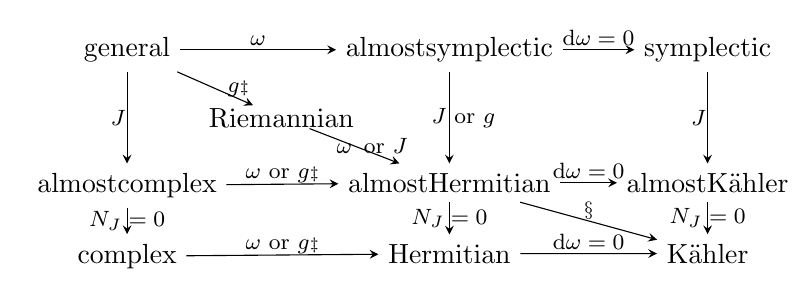
\begin{tikzpicture}
  \matrix (m) [matrix of nodes,row sep=1em,column sep=1em,minimum width=2em] {
     general & & \stackanchor{almost}{symplectic} & & symplectic \\
     & \clap{Riemannian} & & & \\
     \stackanchor{almost}{complex} & & \stackanchor{almost}{Hermitian} & & \stackanchor{almost}{K\"ahler} \\
%     & & & & \\
     complex & & Hermitian & & K\"ahler\\};
  \path[-stealth]
    (m-1-1) edge node [above=-.5ex] {\footnotesize $\omega$} (m-1-3)
    (m-1-1) edge node [right=.1em] {\footnotesize $g$\tabfootsymb{1}} (m-2-2)
    (m-1-1) edge node [left=-.3em] {\footnotesize $J$} (m-3-1)
    (m-1-3) edge node [above=-.5ex] {\footnotesize $\dd{\omega}=0$} (m-1-5)
    (m-1-3) edge node [right=-1em] {\footnotesize $J$ or $g$} (m-3-3)
    (m-1-5) edge node [left=-.3em] {\footnotesize $J$} (m-3-5)
    (m-2-2) edge node [right=-1em] {\footnotesize $\omega$\, or $J$} (m-3-3)
    (m-3-1) edge node [above=-.7ex] {\footnotesize $\omega$ or $g$\tabfootsymb{1}} (m-3-3)
            edge node {\footnotesize $N_J=0$} (m-4-1)
    (m-3-3) edge node [above=-.5ex] {\footnotesize $\dd{\omega}=0$} (m-3-5)
            edge node {\footnotesize $N_J=0$} (m-4-3)
            edge node [above=-.7ex] {\tabfootsymb{2}} (m-4-5)
    (m-3-5) edge node {\footnotesize $N_J=0$} (m-4-5)
    (m-4-1) edge node [above=-.7ex] {\footnotesize $\omega$ or $g$\tabfootsymb{1}} (m-4-3)
    (m-4-3) edge node [above=-.5ex] {\footnotesize $\dd{\omega}=0$} (m-4-5)
    ;
  \pgfresetboundingbox
  \path [use as bounding box] (m-3-1.west |- m-1-3.north) rectangle (m-1-5.east |- m-4-3.south);
\end{tikzpicture}
\end{tab}
(Almost)\,quaternionic/quaternion\-Hermitian/quaternion\-K\"ahler and
(almost)\,hyper\-complex/hyper\-Hermitian/hyper\-K\"ahler manifolds are
defined by replacing~$J$ by a 3d~subbundle of $\End TX$ or by global
sections $J_1,J_2,J_3$ as in the table of $G$-structures.
% ref: math/0307118 classification of "Almost Hermitian Structures and Quaternionic Geometries" (Francisco Martín Cabrera and Andrew Swann)
% ref: math/0105206 useful definitions in "HyperHermitian quaternionic Kähler manifolds" (Bogdan Alexandrov)

\noindent\tabfoot{1}
Since $\Lie{GL}(n,\RR)/\Lie{O}(n)$ is contractible, any manifold admits
(non-canonically) an $\Lie{O}(n)$-structure, namely a smooth choice of
which frames are orthonormal, \ie, a Riemannian metric~$g$.  Similarly
$\Lie{GL}(n/2,\CC)/\Lie{U}(n/2)$ is contractible so almost complex
manifolds admit almost Hermitian structures.

\noindent\tabfoot{2}
An almost Hermitian manifold is K\"ahler if (equivalently) its
$\Lie{U}(n/2)$-structure is $1$-integrable; $\dd{\omega}=0$ and $N_J=0$;
$\nabla\omega=0$; $\nabla J=0$; or the holonomy group is in $\Lie{U}(n/2)$.
Locally, $\omega=\I\del\delbar\rho$ for some real-valued K\"ahler
potentials~$\rho$, and $\omega$~is invariant under K\"ahler transformations
$\rho\to\rho+f(z)+\bar{f}(\bar{z})$.



\paragraph{The holonomy group} at $x\in X$ of a connection~$\nabla$ on a
bundle $E\to X$ is the group of symmetries of~$E_x$ arising from
parallel transport along closed curves based at~$x$.

For Riemannian manifolds~$X$ the holonomy group is defined as that of
the Levi-Civita connection on the tangent bundle.  It is a subgroup of
$\Lie{O}(n)$ \big(or $\Lie{SO}(n)$ for $X$~orientable\big) since
parallel transport preserves orthogonality ($\nabla g=0$).

If the holonomy group acts reducibly on the tangent space then~$X$ is
locally (globally if $X$~is geodesically complete) a product.  Simply
connected~$X$ that are locally neither products nor symmetric spaces (we
give a list later) can have the following special holonomy subgroups of
$\Lie{SO}(n)$
(\href{https://ncatlab.org/nlab/show/Berger\%27s+theorem}{Berger's
  theorem})
\begin{tab}{lll}
  Holonomy & Manifold type & $\dim_{\RR}$\\
  \midrule
  % $\Lie{SO}(n)$ & orientable & $n$ \\
  $\Lie{U}(m)$ & K\"ahler & $2m$ \\
  $\Lie{SU}(m)$ & Calabi--Yau CY$_m$ & $2m$ \\
  \midrule
  $\bigl(\Lie{USp}(2k)\times\Lie{USp}(2)\bigr)/\cyclic{2}$ & quaternionic K\"ahler & $4k$ \\
  $\Lie{USp}(2k)$ & hyperK\"ahler & $4k$ \\
  \midrule
  $\Lie{Spin}(7)$ & $\Lie{Spin}(7)$ manifold & $8$ \\
  $\Lie{G}_2$ & $\Lie{G}_2$ manifold & $7$ \\
\end{tab}
% todo: more at https://en.wikipedia.org/wiki/Holonomy
% todo: perhaps http://projecteuclid.org/euclid.jdg/1090351387 interesting?
%
Note that hyperK\"ahler $\implies$ Calabi--Yau $\implies$ K\"ahler since
$\Lie{USp}(m)\subset\Lie{SU}(m)\subset\Lie{U}(m)$.
In contrast, quaternionic-K\"ahler manifolds are not K\"ahler.

% todo:
% A $\Lie{G}_2$-manifold is a $7$-dimensional manifold with a
% $1$-integrable $\Lie{G}_2\to\Lie{GL}(7)$ structure namely the
% corresponding definite 3-form $\omega$ should be covariantly constant
% with respect to the induced Riemannian metric (due to
% $\Lie{G}_2\subset \Lie{SO}(7)$.  Equivalently it is a Riemannian $7$-manifold
% with holonomy group~$\subseteq\Lie{G}_2$.
%
% Example: Aloff--Wallach space $X_{k,l}=\Lie{SU}(3)/\Lie{U}(1)_{k,l}$ where $\Lie{U}(1)\contains\rme^{\I\theta}\mapsto\diag(\rme^{\I k\theta},\rme^{\I l\theta},\rme^{\I(-k-l)\theta})\in\Lie{SU}(3)$ have many $\lie{G}_2$-structures.

A \href{http://en.wikipedia.org/wiki/Calabi-Yau_manifold}{Calabi--Yau
  manifold} is a K\"ahler manifold such that (equivalently) some
K\"ahler metric has global holonomy group in $\Lie{SU}(m)$; the
structure group can be reduced to $\Lie{SU}(m)$; or the holomorphic
canonical bundle is trivial \ie, there exists a nowhere vanishing
holomorphic top-form.  A weaker set of equivalent conditions

\todo{here}

For simply connected manifolds, the conditions above are equivalent to
the following (always equivalent) conditions on~$X$: some K\"ahler
metric has local holonomy group in $\Lie{SU}(m)$; some K\"ahler metric
has vanishing Ricci curvature; the first real Chern class vanishes; a
positive power of the holomorphic canonical bundle is trivial; $X$~has a
finite cover with trivial holomorphic canonical bundle; $X$~has a finite
cover equal to the product of a torus and a simply connected manifold
with trivial holomorphic canonical bundle.

% todo: every Kähler manifold is spin (or at least spinc)

% todo: every hyperKähler manifold is Ricci-flat

% todo: every hyperKähler manifold is Calabi--Yau

% todo: ``Calabi proved a partial converse which says that a compact holomorphically symplectic Kähler manifold admits a unique hyperKähler metric with respect to any of its Kähler forms.'' (Mathworld)

% todo: more on http://mathworld.wolfram.com/Hyper-KaehlerManifold.html

% todo: more on Laplacians on Kähler manifolds at Wikipedia

% todo: HyperK\"ahler manifolds admit holomorphic symplectic forms (i.e. non-degenerate closed holomorphic $2$-form) $\omega_2+\I\omega_3$

% todo: Kodaira's classification of complex surfaces

% todo: complex submanifold of a Kähler manifold is Kähler, in particular projective algebraic varieties and Stein manifolds

% todo: Einstein manifold R=λg (but is λ constant?)

% todo: Kähler--Einstein manifold

% todo: self-dual Einstein manifolds

% Every quaternionic-K\"ahler manifold is locally almost hypercomplex

% Every quaternionic-K\"ahler manifold is Einstein

% A quaternionic-K\"ahler with zero scalar curvature is locally hyperK\"ahler

% Compact hyperHermitian $4$-manifolds are conformal to tori, Hopf or K3. [ DOI: 10.2307/2046051 , Stable URL: http://www.jstor.org/stable/2046051 ]

\paragraph{Spin structures} \todo{see\quad \url{http://mathoverflow.net/questions/220502/}}

\paragraph{Symmetric spaces} \todo{list missing}

% todo: symmetric spaces? https://en.wikipedia.org/wiki/Symmetric_space

\paragraph{K3 surfaces} are the only CY$_2$: they have holonomy
$\Lie{SU}(2)$.

\paragraph{Yau's theorem.}  Fix a complex structure on a compact complex
manifold~$X$ of $\dim_{\CC}X>1$ and vanishing real first Chern class.
Any real class $H^{1,1}(X,\CC)$ of positive norm contains a unique
K\"ahler form whose metric is Ricci flat.

(from Wikipedia on Calabi conjecture: ``The Calabi conjecture states that a compact Kähler manifold has a unique Kähler metric in the same class whose Ricci form is any given 2-form representing the first Chern class.'')

% \subsection{Misc properties of manifolds}

% todo \paragraph{Rokhlin's theorem}


\section{Misc}

\subsection{Physics of gauge theories}

\paragraph{Phases characterized by potential} $V(R)$ (up to a constant) between quarks at distance~$R$:
Coulomb $1/R$,
free electric $1/\bigl(R\log(R\Lambda)\bigr)$,
free magnetic $\log(R\Lambda)/R$,
Higgs (constant),
confining $\sigma R$.

\paragraph{Instantons}
are anti-self-dual ($F=-{\star F}$) connections on~$\RR^4$ that decay at infinity and extend to~$S^4$.
The bundles are classified by $\pi_3(G)$ so an instanton number $k\in\ZZ$ for simple gauge groups;
for fixed $k\geq 0$ ($k\leq 0$) (anti)instantons minimize the action.
The $k$-instanton moduli space for $G=\Lie{SU}(N)$ is a $4Nk$-dimensional \inspire{128223} hyperK\"ahler manifold,
in bijection with rank~$N$ framed locally free sheaves on~$\CC\PP^2$ \inspire{125044}.

\subsection{Homology and cohomology}

\paragraph[Complex projective space]{$H_k(\CC\PP^n,M)$}${}=M$ for $0\leq k\leq 2n$ even, else~$0$.

\subsection{Homotopy groups \(\pi\sb n\)}

\paragraph{Basic properties.} $\pi_0(X,x)$ is the set of connected components.  $\pi_1(X,x)$ is the fundamental group.  For $k\geq 1$, $\pi_k(X,x)$ only depends on the connected component of~$x$.  $\pi_k(X\times Y,(x,y))=\pi_k(X,x)\times\pi_k(Y,y)$.

\paragraph{Quotient.}  If $G$~acts on connected simply-connected~$X$ then $\pi_1(X/G)=\pi_0(G)$ ($=G$ for $G$~discrete).

\paragraph{Long exact sequence for a fiber bundle} $F\hookrightarrow E\twoheadrightarrow B$: for base-points $b_0\in B$ and $e_0=f_0\in F=p^{-1}(b_0)\subset E$, $\cdots\to\pi_{i+1}(B)\to\pi_i(F)\to\pi_i(E)\to\pi_i(B)\to\cdots\to\pi_0(E)$ is exact, namely each image equals the next kernel (inverse image of the constant map).

\paragraph{Homotopy groups of spheres} are finite except $\pi_n(S^n)=\ZZ$ and $\pi_{4n-1}(S^{2n})=\ZZ\times\text{finite}$.  For $k<n$, $\pi_k(S^n)=0$, and $\pi_{n+k}(S^n)$ is independent of~$n$ for $n\geq k+2$.  All $\pi_k(S^0)=0$, $\pi_k(S^1)=0$ for $k\neq 1$, and $\pi_k(S^3)=\pi_k(S^2)$ for $k\neq 2$.
\begin{tab}{*9{>{$}c<{$}}}
  & \pi_1 & \pi_2 & \pi_3 & \pi_4 & \pi_5 & \pi_6 & \pi_7 & \pi_8 \\\midrule
  S^0 & 0 & 0 & 0 & 0 & 0 & 0 & 0 & 0 \\
  S^1 & \ZZ & 0 & 0 & 0 & 0 & 0 & 0 & 0 \\
  S^2 & 0 & \ZZ & \ZZ & \ZZ_2 & \ZZ_2 & \ZZ_{12} & \ZZ_2 & \ZZ_2 \\
  S^3 & 0 & 0 & \ZZ & \ZZ_2 & \ZZ_2 & \ZZ_{12} & \ZZ_2 & \ZZ_2 \\
  S^4 & 0 & 0 & 0 & \ZZ & \ZZ_2 & \ZZ_2 & \ZZ\times \ZZ_{12} & \ZZ_2^2 \\
  S^5 & 0 & 0 & 0 & 0 & \ZZ & \ZZ_2 & \ZZ_2 & \ZZ_{24} \\
\end{tab}
% data of the table found on Wikipedia page
$\pi_1(\RR\PP^n)=\ZZ_2$ for $n\geq 2$ and $\pi_k(\RR\PP^n)=\pi_k(S^n)$ for $k\geq 2$.
$\pi_1(\CC\PP^n)=0$, $\pi_2(\CC\PP^n)=\ZZ$, $\pi_k(\CC\PP^n)=\pi_k(S^{2n+1})$ for $k\geq 3$.

\paragraph{Topological groups have abelian \(\pi\sb 1(G)\).}
% http://mathoverflow.net/questions/35868/fundamental-group-of-lie-groups
Proofs.  1.\@ The multiplication in~$G$ (point-wise) and concatenation of loops are two compatible group structures, hence (by Eckmann--Hilton theorem) coincide and are commutative.  2.\@ Explicitly, for $\alpha_1,\alpha_2\in\pi_1(G)$ loops, $(t_1,t_2)\mapsto\alpha_1(t_1)\alpha_2(t_2)\in G$ is a homotopy between $\alpha_1\star\alpha_2$ (concatenation) along bottom and right edges, $\alpha_1\cdot\alpha_2$ (point-wise multiplication) along the diagonal, and $\alpha_2\star\alpha_1$ along left and top edges.

\subsection{K\"ahler \(4\)-manifolds}
 % see 1206.1070 for detailed exposition

\paragraph{K3~surfaces} are (the only besides~$T^4$) compact complex
surfaces of trivial canonical bundle.  They have $h^{1,0}=0$ (in
contrast to~$T^4$ which has \todo{value}).  Their first Chern class
$c_1\in H^2(X,\ZZ)$ thus vanishes.  By Yau's theorem there exists a
Ricci flat metric, whose holonomy is then $\Lie{SU}(2)=\Lie{USp}(2)$ by
Berger's classification.
% todo: which Sp?
K3~surfaces are thus Calabi--Yau (CY$_2$) and hyperK\"ahler (hK$_4$).
Their moduli space is connected and they are all diffeomorphic.

\paragraph{Examples of K3~surfaces.} Quartic hypersurface in~$\PP^4$.
Kummer surface namely resolution of $T^4/\cyclic{2}$.

% todo: maybe move closer to Yau's theorem in "Types of manifolds"?
\paragraph{Non-simply connected} Ricci-flat K\"ahler manifolds may fail
to be CY$_n$ when the restricted holonomy group is $\Lie{SU}(n)$ but the
global holonomy group is disconnected.  For example an Enriques surface
K3$/\cyclic{2}$ has a non-trivial canonical bundle.

\paragraph[Gravitational instantons]{A gravitational instanton} is a
metric with (anti-)self-dual curvature.  A simply-connected Riemannian
4-manifold is hyperK\"ahler if and only if it is a gravitational
instanton.  Compact hK$_4$ are K3 and~$T^4$.  Non-compact hK$_4$ are ALE
(asymptotically locally Euclidean), ALF (asymptotically locally flat),
ALG, ALH if their volume growth rate is of order $4$, $3$, $2$, $1$.
ALE spaces are resolutions of $\HH/\Gamma$ for a finite subgroup
$\Gamma<\Lie{USp}(2)$.  The quotient $\HH/\Gamma$ can appear as a local
model of an orbifold singularity in a K3~surface.

% \arxiv{1505.01790}

\paragraph{ALE hyperK\"ahler \(4\)-manifolds} $X$ are
diffeomorphic to the minimal resolution of $\HH/\Gamma$ for some finite
$\Gamma\subset\Lie{SU}(2)$.  The metric is fixed (up to isometry) by
cohomology classes $\alpha_1,\alpha_2,\alpha_3\in H^2(X,\RR)$ such that
there is no two-cycle~$\Sigma$ such that $\Sigma\cdot\Sigma=-2$ and all
$\alpha_i(\Sigma)=0$.
% todo: cite Kronheimer, The construction of ALE spaces as hyper-Kähler quotients

\todo{Taub-NUT spaces, multi-Taub-NUT spaces,
  Eguchi--Hanson spaces, Gibbons--Hawking multicenter spaces.  Write
  metric.}  \todo{Non-explicitly: Atiyah--Hitchin space (moduli space of
  two $\Lie{SU}(2)$ 't~Hooft-Polyakov monopoles in~4d).}

\todo{The only compact CY$_2$ are $T^4$ and K3~surfaces.}

\todo{The only compact hypercomplex $4$-manifolds are $T^4$,
  K3~surfaces, and the Hopf surface ($(\HH\setminus 0)/(q^\ZZ)$ for a
  quaternion $\abs{q}>1$; it is diffeomorphic to $S^3\times S^1$).}

% todo: what is the (co)homology of $X\times Y$?

% todo: In\"on\"u--Wigner contraction (for Lie superalgebras too)

% todo: vortices, monopoles, instantons (Abrikosov--Nielsen--Olesen
% vortex, 't~Hooft--Polyakov monopole, \ldots{}).

\subsection{Some algebraic constructions}

\paragraph{Reduction of a Lie (super)algebra}~$\lie{G}$.  If $\lie{G}=V_1\oplus V_2$ with $[V_1,V_2]\subseteq V_2$ then the bracket of~$\lie{G}$ restricted and projected to~$V_1$ defines a Lie (super)algebra.

\paragraph{\(S\)-expansion of a Lie (super)algebra}~$\lie{G}$ by an abelian multiplicative semigroup~$S$: Lie (super)algebra $\lie{G}\times S$ with bracket $[(x,\alpha),(y,\beta)]=([x,y],\alpha\beta)$.  If $S=S_1\cup S_2$ with $S_1 S_2\subseteq S_2$ (in particular if there is a zero element $0_S=0_S\alpha=\alpha 0_S$) then by reduction we get a Lie (super)algebra structure on $\lie{G}\times S_1$.

\paragraph{A color (super)algebra} is a graded vector space with a bracket such that (for $X$, $Y$, $Z$ with definite grading) $\gr [X,Y] = \gr X+\gr Y$ and $[X,Y]=-(-1)^{(\gr X,\gr Y)}[Y,X]$ and Jacobi identity $[X,[Y,Z]](-1)^{(\gr Z,\gr X)}+[Y,[Z,X]](-1)^{(\gr X,\gr Y)}+[Z,[X,Y]](-1)^{(\gr Y,\gr Z)}=0$, where $(\bullet,\bullet)$ is some bilinear mapping into $\CC/(2\ZZ)$.

\subsection{Other}

\paragraph[Fuzzy spaces]{A fuzzy space} is $d$~Hermitian matrices~$X^a$ (``coordinates'') acting on some Hilbert space~$H$.  The dispersion of $\psi\in H$ is $\delta_\psi=\sum_a\bigl(\langle\psi\rvert (X^a)^2\lvert\psi\rangle-\langle\psi\rvert X^a\lvert\psi\rangle^2\bigr)$.

% =============================
% Other interesting things to talk about
% https://en.wikipedia.org/wiki/Genus_of_a_multiplicative_sequence

\bigskip
\vfill
\setlength{\parindent}{0pt}

\end{document}
